\documentclass[times, utf8, zavrsni, numeric]{fer}
\usepackage{booktabs}
\usepackage{url}
\usepackage[final]{pdfpages}
\usepackage{amsmath}
\usepackage{blindtext}
\usepackage{enumitem}
\usepackage{listings}
\usepackage[hidelinks]{hyperref}

\renewcommand{\lstlistingname}{Programski isječak}% Listing -> Algoritam
\renewcommand{\lstlistlistingname}{Popis programskih isječaka}% List of Listings -> Popis algoritama 

\lstdefinestyle{mystyle} {
	basicstyle=\footnotesize,
	numbers=left,
	numberstyle=\tiny,
	frame=tb,
	columns=fullflexible,
	showstringspaces=false
	breakatwhitespace=false,         
	breaklines=true,                 
	captionpos=b,                    
	keepspaces=true,                 
	numbersep=5pt,                  
	showspaces=false,                
	showtabs=false,                  
	tabsize=4,
	inputencoding=utf8,
	morekeywords={vrati, ako, inače, za\_svaku, za\_svaki, prekini\_petlju, dok, funkcija} 
}	

\lstset{style=mystyle,texcl=true}
% set font translations
%\lstset{inputencoding=utf8}
\lstset{extendedchars=true}
\lstset{
	literate=%
	{ć}{{\'c}}1
	{č}{{\v{c}}}1
	{đ}{{\dj{}}}1
	{š}{{\v{s}}}1
	{ž}{{\v{z}}}1
	{Ć}{{\'C}}1
	{Č}{{\v{C}}}1
	{Đ}{{\DJ{}}}1
	{Š}{{\v{S}}}1
	{Ž}{{\v{Z}}}1
}

\begin{document}

% TODO: Navedite broj rada.
\thesisnumber{5173}

\title{Implementacija jezgre RTS igre}

\author{Leon Luttenberger}

\maketitle

% Ispis stranice s napomenom o umetanju izvornika rada. Uklonite naredbu \izvornik ako želite izbaciti tu stranicu.
\izvornik{}

% Dodavanje zahvale ili prazne stranice. Ako ne želite dodati zahvalu, naredbu ostavite radi prazne stranice.
\zahvala{}

\tableofcontents

\chapter{Uvod}

\par Računalne igre predstavljaju vrlo značajan pokretač razvoja računala.
Jednu zanimljivu vrstu igara čine strategije u stvarnom vremenu (engl. \textit{Real-Time Strategy}, RTS).
U njima igrač mora poraziti protivnike razmišljanjem i donošenjem prikladnih taktičkih odluka, te je utjecaj vjerojatnosti minimalan.
U okviru ovoga rada istraženi su i implementirani nezavisni podsustavi RTS-igre te je izrađen prototip jedne konkretne RTS-igre.

\par U~\ref{ch:games}.~poglavlju napravljen je kratak pregled različitih vrsta računalnih igara i osnovnih podsustava prisutnih u njima.

\par U~\ref{ch:rtsGames}.~poglavlju izrađen je detaljnih opis žanra igara RTS.
Ovdje su istraženi osnovni podsustavi koji se nalaze u takvim igrama i nisu specifični za konkretnu igru već se mogu višestruko iskorištavati.

\par Jedan od podsustava prisutnih u svim igrama RTS je samostalno kretanje jedinica. 
Teorijska podloga ovog podsustava je detaljnije istražena u~\ref{ch:pathfinding}.~poglavlju.
U tom su poglavlju prikazani postupci pretraživanja stanja u statičkom okruženju.
Budući da se RTS-igre održavaju u dinamičkom svijetu, te je postupke potrebno prilagoditi kako bi se i oni sami mogli prilagođavati promjenama u svijetu igre.

\par Zatim je napravljena programska implementacija osnovnih podsustava koji se mogu dijeliti između različitih igara RTS.
Također je izrađena konkretna implementacija jednog prototipa RTS-igre koji sadrži osnovne elemente poput prikaza mape svijeta, stvaranja građevina i jedinica, osnovnih protivničkih jedinica te upravljanje vlastitim jedinicama.
Upravljanje vlastitim jedinicama uključuje grupiranje, zadavanje ciljeva, pucanje i prikupljanje resursa.

\par Programska implementacija osnovnih podsustava i konkretnog prototipa opisana je u~\ref{ch:implementation}.~poglavlju.
Nadalje, opisan je postupak jednostavnog dodavanja novih funkcionalnost u konkretnu igru koje nisu ovisne o navedenoj igri.

\chapter{Pregled vrsta računalnih igara}\label{ch:games}

\par Klasifikacija žanrova računalnih igara nije strogo određena.
Svaka igra može se klasificirati po osobnim kriterijima te može pripadati više od jednom žanru istovremeno.
U ovom poglavlju napravljen je kratak pregled nekoliko najbitnijih žanrova koji se međusobno bitno razlikuju po svom utjecaju i podsustavima.

\section{Platformeri}

\par Platformeri su jedan od starijih žanrova računalnih igara.
One su tipično prikazane u 2D svijetu, u kojima igrač započne igru na dnu ekrana i cilj je pomoću pravovremenih skokova po platformama popeti se na vrh.
Na putu do cilja, igrač će susresti protivničke jedinice koje je cilj izbjeći.

\par Zbog ograničenosti računala u doba kada je ovaj žanr nastao, protivničke jedinice su strogo skriptirane, npr.\ beskonačno se kreću lijevo-desno po svojoj platformi.
Kao posljedica toga, igranje ovakvih igra se pretežno svodi na predviđanje idućih događaja u igri.

\section{Žanr RPG}

\par Kada su osobna računala postala šire dostupna, računalne igre su počele iskorištavati kompleksniji sustav kontrola koje su omogućili miš i tipkovnica u odnosno na dotadašnje igraće palice (engl. \textit{joystick}).
Žanr igara poznat pod nazivom RPG\footnote{Igre igranja uloga (engl. \textit{Role playing games})} je nastao u to vrijeme.
Dotadašnje igre su uglavnom bili portovi arkadnih igara, poput \textit{Pacmana} ili \textit{Asteroids}.
Mana kod takvih igara je što su bile dizajnirane da kratko traju kako bi igrača natjerale da često ubacuje kovanice u igraći automat, zbog čega su se RPS igre isticale sa svojim trajanjem.

\par U RPG igrama igrač tipično kontrolira jednog lika koji krene ni sa čime, obavlja razne poslove za novac, trenira svoje sposobnosti i s vremenom postaje sve moćniji. 
Neovisno o detaljima specifične igre, ideja svih igara u ovom žanru je omogućiti igraču da se poistovjeti s glavnim likom i unese u svijet u kojem se glavni lik nalazi.

\par Likovi u ovakvih igrama se tipično dijele u obične neprijatelje, ''\textit{šefove}'' i pasivne \textit{NPC}\footnote{Ne-igraći likovi         
(engl. \textit{Non-playable characters})} jedinice.
Obični neprijatelji su najčešći tip likova.
Njihova svrha je boriti se protiv igrača, te ih tipično ima u beskonačnoj količini kako bi igrač uvijek imao nešto za raditi.
''\textit{Šefovi}'' generalno predstavljaju vođe protivničkih skupina, i kompleksniji su i teži protivnici koji se pojavljuju na kraju svake razine ili sekcije nakon što igrač porazi mnogo slabijih protivnika.
Zamišljeni su kako bi iznenadili igrača sa svojom moći i razbili monotonost igre.
\textit{NPC} prema strogoj definiciji predstavlja svaku jedinicu koja nije pod kontrolom igrača. 
Međutim, termin se najčešće koristi za likove u igri s kojima igrač može imati interakciju osim borbe, poput stanovnika grada ili nasumičnih likova koje igrač sretne tijekom igre.

\par Kako bi se svijet u kojem se igra odvija činio što stvarniji, likovi u svijetu se također moraju ponašati što realnije.
Kao posljedica toga i čistog dosega ovakvih igara, one znaju imati vrlo visoke standarde za umjetnu inteligenciju.
Primjerice, ako igrač posjeti neko selo ili grad u svijetu igre, ono mora biti ispunjeno s ljudima koji imaju svoje živote, pozadinu i posao.
Dodatna doza uvjerljivosti se postigne ako \textit{NPC}-ovi u tom gradu svaki dan ujutro odu na posao, na kraju radnog dana otputuju kući i po noći spavaju.
Navedena funkcionalnost lako je izvediva uporabom nedeterminističkih konačnih automata~\cite{book:AIGameProgrammingWisdom}.

\section{Žanr pucačina}

\par Postoje dvije glavne vrste pucačina: pucačine iz prvog lica, poznate kao FPS\footnote{engl. \textit{First person shooter}}, i pucačine iz trećeg lica, poznate kao TPS\footnote{engl. \textit{Third person shooter}}.
U pucačinama iz prvog lica igrač svijet promatra iz perspektive lika kojeg kontrolira, odnosno kamera se nalazi tamo gdje su njegove oči.
Suprotno tome, u pucačinama iz trećeg lika kamera se nalazi iza glavnog lika što omogućava igraču da može vidjeti model svog lika.
Bez obzira na igračevu perspektivu u ovakvim igrama, njihova premisa je vrlo jasna.
Igrač kontrolira lika koji u rukama drži nekakvo vatreno oružje te se mora boriti protiv neprijatelja.

\par Igre u ovom žanru su igrale ključnu ulogu u podizanju standarda za grafičke i mrežne performanse u računalnim igrama.
Također, kako bi bitke u igri bile što zahtjevnije, bitnu ulogu igra i razvoj botova, odnosno autonomnih agenta koji znaju pronaći svoj put na mapi, tražiti neprijatelje, skupljati oružja i boriti se.
Umjetna inteligencija iza navedenih botova je obično modelirana zasebno, kako sama igra ne bi direktno ovisila o specifičnoj implementaciji.
To svojstvo omogućava proširivost same igre, odnosno omogućava programerima da napišu svoje implementacije te ih testiraju u samoj igri.

\par Zahvaljujući navedenom svojstvu, neke igre u ovom žanru se često koriste u istraživanjima umjetne inteligencije.
Uvjeti u takvim igrama mogu biti puno bliži uvjetima u stvarnom svijetu nego čisti laboratorijski uvjeti, što omogućava učinkovito ispitivanje novih i bržih algoritama.

\section{Sportske igre}

\par Prva računalna igra ikad napravljena je bila \textit{Pong}, odnosno vrlo jednostavna verzija tenisa.
Igre u ovom žanru duguju svoju popularnost prepoznatljivosti vlastitih pravila i mehanike.
Primjerice, igra o nogometu imat će ista pravila kao i nogomet u stvarnom svijetu, te se zbog toga ovakve igre ne moraju posebno ''učiti''.

\par U prošlosti, umjetna inteligencija u sportskim igrama bila je skriptirana što je igračima omogućavalo da jednostavno prate uzorke i predviđaju sljedeće poteze, kao i u platformerima.
Danas igrači ovakvih igara očekuju da se računalni protivnici znaju dobro dovoljno dobro igrati igru da budu izazov i za najiskusnije igrače.
Naglasak ovdje je na igre u kojima umjetna inteligencija postiže svoj uspjeh pametnim igranjem, umjesto da ''vara'' tako da si umjetno povećava statistike, poput šansa za pogodak.

\par U ovaj žanr mogu se svrstati i trkaće igre.
U trkaćim igrama igrač sudjeluje u nekakvoj vrsti utrke, poput auta, aviona, glisera, svemirskih brodova, itd.
Spektar realnosti u ovakvim igrama je vrlo širok, odnosno neke igre se strogo drže zakona fizike iz stvarnog svijeta kako bi sama vožnja bila što veći izazov, dok ih ostale slobodno interpretiraju kako bi igraču ponudile jedinstveno iskustvo i ugođaj.

\section{Strategije}

\par Strategije su žanr računalnih igara u kojima igrač ima kontrolu nad svim aspektima borbe i razvoja te mu je tipično cilj minimizirati količinu neprijateljskih jedinica.
Ključ pobjede je planirati niz akcija s kojima će se nadmudriti protivnike.

\par U većini igara u ovom žanru, igrač ima pogled odozgora na čitav teren i indirektno upravlja svojim jedinicama, odnosno daje im naredbe gdje da se kreću bez da on mora sam kontrolirati kretanje.
Igrač zato direktno upravlja višim strateškim i taktičkim odlukama, poput ekonomskog i tehnološkog razvoja svoje strane.

\par Igre u ovom žanru mogu se podijeliti u dvije kategorije: strategije u stvarnom vremenu (RTS) i strategije na potez (engl. \textit{Turn-based strategy}).
U strategijama u stvarnom vremenu igra vrijeme konstantno teče te igrači svi istovremeno kontroliraju svoje strane.
U strategijama na potez, tijek igre je analogan tijeku igre u klasičnim strategijama poput šaha, odnosno igrači više ne igraju u isto vrijeme.
Kao posljedica toga, u strategijama na potez nije bitna brzina razmišljanja i reakcije igrača, već je naglasak na dugoročno planiranje i nadmudrivanje protivnika.

\par U nastavku ovog rada detaljnije su opisani aspekti RTS-igara.

\chapter{Igre RTS}\label{ch:rtsGames}

\par Računalne igre svrstane pod žanr RTS temelje se na skupljanju resursa za izgradnju jedinica i građevina s ciljem da se poraze protivnici. 
Za razliku od strategija na potez gdje svaki igrač ima proizvoljno vrijeme za odigrati svoj potez, u RTS-igrama svi igrači igraju u isto vrijeme.
Dodatna napetost nastaje zbog znanja da svi ostali igrači aktivno pokušavaju ostvariti svoje ciljeve i spriječiti sve ostale igrače u rađenju istoga.
U širem smislu, RTS-igra se može definirati kao simulacija bitke u stvarnom vremenu.

\section{Elementi žanra RTS}

\par Tipična RTS-igra sastoji se od mnogih različitih elemenata.
Prije svega, svaka igra se odvija na mapi ograničene veličine koja je određena s raznim tipovima terena, poput trave, vode, planina, pustinje, itd. 
Tip terena može odrediti koje se jedinice mogu kretati po njemu.
Primjerice, pravila igre mogu biti takva da se običan vojnik ne može kretati po vodi, dok neki drugi tip jedinice poput broda može.
Kao posljedica toga, teren igra veliku ulogu jer od igrača pozicija može zahtijevati korištenje posebnih strategija.

\par Još jedna bitan element RTS-igara je skupljanje resursa.
Ovisno o konkretnoj igri, resursi mogu biti drvo, minerali, nafta, zlato, itd. Oni se tipično skupljaju s posebnom vrstom jedinica zvanom radnicima, te se koriste za izgradnju novih jedinica, zgrada, itd.
Resursi također igraju veliku ulogu u strategiji same igre.
Primjerice, ako se igrač nalazi u situaciji gdje ne može dalje napredovati zbog manjka nekog resursa, bit će prisiljen otići u potragu za istim.
Analogno tome, višak izvora nekog resursa igrača može postaviti u opasnost jer će ostalim sudionicima igre biti prioritet napasti s ciljem preuzimanja resursa.

\par Osim resursa i mape, bitan element u svakoj RTS-igri je izgradnja zgrada. 
Konkretne igre obično imaju mnogo različitih zgrada od kojih svaka ima svoj skup funkcionalnosti, poput treniranja novih jedinica, procesiranje resursa, istraživanje novih tehnologija, itd.  

\par Posljednji bitni element igara u žanru RTS su jedinice. 
Svaka igra ima skup različitih jedinica koje igrač može odabrati i izgraditi za svoju vojsku.
Svaka vrsta jedinice može imati svoje prednosti i mane.
Npr.\ igra može kao vrstu jedinice imati konjanika koja ima prednost brzog kretanja po mapi, no ima manu da je izrazito ranjiv na kopljanike.

\par Jedna od posebnosti žanra RTS je činjenica da svi dosad navedeni elementi nisu direktno ovisni jedni o drugima.
Mapa može biti definirana izvan same igre u nekom vanjskom uređivaču mapa, dok jedinice, resursi i zgrade ne moraju ništa konkretno znati jedni o drugima.
Jedinice će samo znati da se kreću po terenu koji ima neke definirane karakteristike, te će samo znati da napada protivničke zgrade i jedinice. 
Zgrade i resursi mogu biti definirani samo kao objekti na mapi, gdje će bilo kakva daljnja funkcionalnost ovisiti o konkretnoj igri.

\par Takva struktura može omogućiti da se određene komponente iz igre višestruko iskorištavaju te da se nove funkcionalnosti mogu lakše dodavati u igru.
Primjer ovakve strukture implementiran je u okviru ovoga rada, te su detalji više obrađeni u poglavlju~\ref{ch:implementation}.

\section{Strategija}

\par Glavni cilj u igrama u žanru RTS analogan je igrama poput šaha, odnosno cilj je pametnom uporabom vlastite vojske poraziti vojsku od suparnika. 
Za razliku od šaha, u računalnim strateškim igrama igrač započne igru ''praznih ruku'', odnosno igru može započeti sa samo jednim radnikom čiji je posao skupiti prve resurse s kojima će izgraditi prve jedinice te nove radnike i zgrade.

\par Igrač jedinicama daje naredbe tako da ih odabere (npr.\ pritiskom tipke miša) i zada im odredište gdje se moraju pomaknuti ili protivničku jedinicu koju moraju napasti. 
Igrač također može odabrati zgradu i njoj dati naredbu što da proizvodi, poput novih jedinica ili istraživanja novih tehnologija koje će omogućiti izgradnju novih tipova jedinica i zgrada.

\par Odluke u igrama RTS mogu se podijeliti u dvije kategorije: mikro-upravljanje i makro-upravljanje. 
Makro-upravljanje predstavlja odluke na višoj razini apstrakcije poput odluka koje zgrade i jedinice graditi, kada krenuti u napad, itd. 
Mikro-upravljanje svodi se na upravljanje pojedinim jedinicama.
Dobro taktičko pozicioniranje jedinica i fokus na najjače protivničke jedinice u dosegu često mogu definirati ishod igre~\cite{article:HybridPathdinding}.

\par Kao posljedica svega navedenog, evidentno je da je strategija centralnih aspekt igara u žanru RTS.

\par Također, bitno je naglasiti da će određene strategije funkcionirati samo protiv pojedinih protivnika i da određene situacije mogu zahtijevati promjenu strategije. 
Primjerice, igrač se može odlučiti za strategiju ranog napada (engl. \textit{rush strategy}), odnosno odmah se fokusirati na izgradnju velikog broja osnovnih borbenih jedinica koje će što ranije moguće poslati u napad na protivnika.
Kao kontrast tome, protivnik se može fokusirati na razvoj tehnologije što će ga ostaviti ranjivim na početku igre, ali će mu u kasnijim fazama igre omogućiti da gradi jedinice koje su jače od protivničkih.

\section{Izazov za umjetnu inteligenciju}

\par RTS-igre predstavljaju razne izazove za razvoj umjetne inteligencije. 
Iz perspektive mikro-upravljanja, umjetna inteligencija mora imati sustav po kojem će određivati najkraći put do odredišta, te kako se treba ponašati u slučaju da na putu naiđe na nešto neplanirano, poput protivničkih jedinica ili promjena na terenu. 
S druge strane, makroupravljanje je mnogo složeniji izazov za umjetnu inteligenciju jer sustav mora odrediti dugotrajne ciljeve, npr.\ hoće li se fokusirati na jaku vojsku, tehnološki ili ekonomski razvoj, itd.

\par Navigacija jedinica je u igrama RTS često najintenzivniji posao za centralni procesor računala.
Veliki broj jedinica stvara potrebu za velikim brojem pretraga, pogotovo ako se svaka kreće u svom smjeru, te svaka od njih mora pratiti potencijalne promjene na terenu i promijeniti ponašanje u skladu s istima.
Tehnike poput skupljanja jedinica u grupe kako bi se zajedno kretali prema cilju mogu smanjiti taj trošak, jer će se sve pretrage i provjere izvršavati nad tom grupom jedinica~\cite{book:AIGameProgrammingWisdom}. 

\par Na slici~\ref{fig:RTSgrouping} prikazane su tri jedinice kako se zajedno kreću prema bijeloj liniji koja označava najkraću putanju.
Pretraga je obavljena za čitavu grupu odjednom, umjesto za sve jedinice zasebno, što je značajno smanjilo trošak izračuna puta.

\begin{figure}[h] 
	\centering
	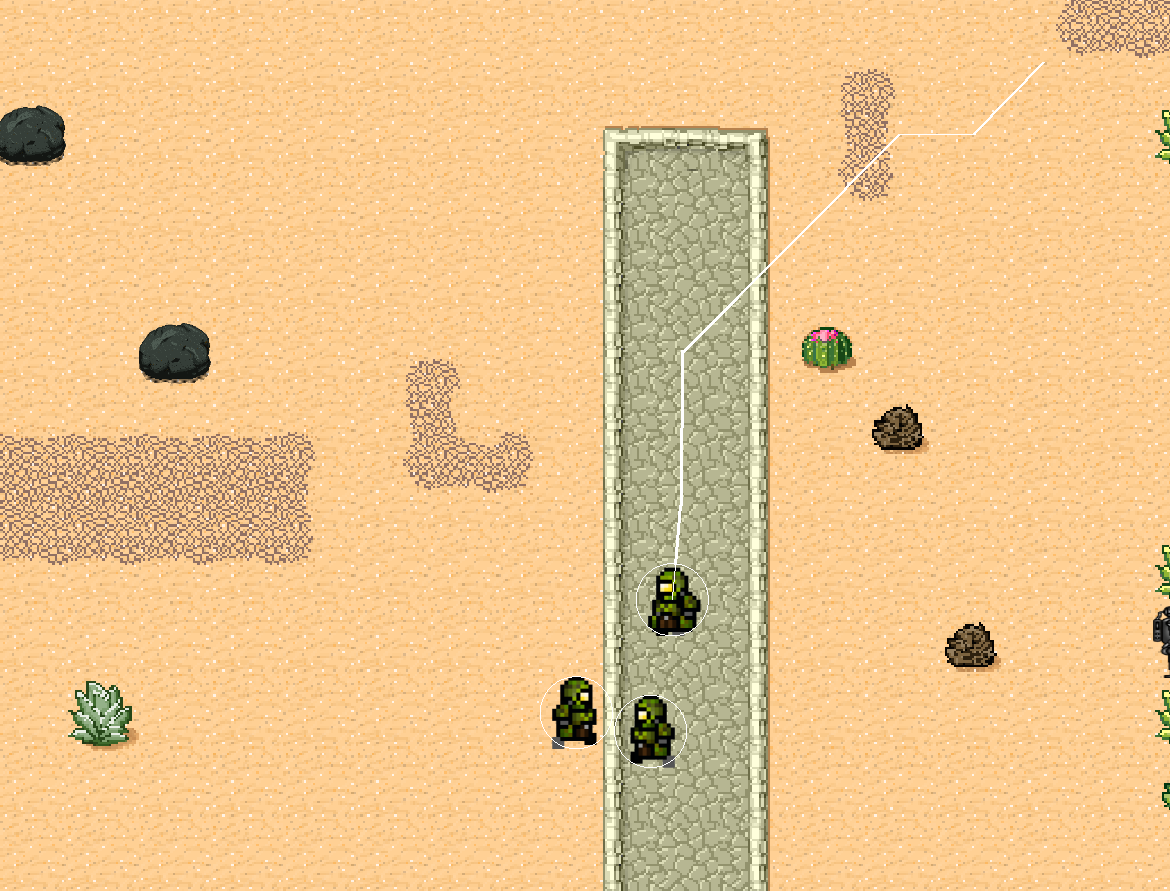
\includegraphics[width=0.6\linewidth]{images/RTSgrouping.png}
	\caption{Zajedničko kretanje jedinica}
	\label{fig:RTSgrouping}
\end{figure} 

\par Jedinice se također moraju znati ponašati u borbi na što pametniji način. Primjerice, strijelac bi se trebao držati na udaljenosti od mete jer je tamo najopasniji.
U trenutku kada se nađe u borbi prsa u prsa, njegova najbolja strategija je povući se na udaljenost iz koje može pucati.
Međutim, osposobiti i igračeve jedinice da se automatski ponašaju na navedeni način  je dvosjekli mač.
S jedne strane, jedinice će biti sposobnije i igrač neće morati konstantno mikro-upravljati njima.
Međutim, navedenu prednost će neki igrači smatrati manom.
Ako su strijelci dovoljno pametni da se znaju držati na udaljenosti iz koje mogu pucati i povlače se kada dođu u opasnost, to eliminira potrebu za nekim strategijama s kojima su dugogodišnji igrači strategija dobro upoznati.
Primjer takve strategije je napraviti formaciju strijelaca tako da budu u jednoj liniji, te između njih i neprijatelja postaviti mačevalce koji će sprječavati protivnike da se približe.

\par Umjetna inteligencija koja će upravljali strategijom na višoj razini slična je ulozi generala u vojsci. 
Ona dobiva percepcije o trenutnom stanju na terenu od njenih jedinica.
Na temelju tih percepcija računalo može bitno promijeniti trenutnu strategiju. Primjerice, ako je računalo negdje otkrilo izvore resursa, ono može napraviti odluku da radnike pošalje u tom smjeru kako bi skupili što više toga.
Nadalje, ako se taj resurs može koristiti za razvoj tehnologije, u trenutku kada ga se skupi dovoljno računalo može promijeniti dugotrajni cilj u igri na tehnološki razvoj.

\par Dugotrajni ciljevi mogu ovisiti i o tome s kojom se frakcijom igra. 
Npr.\ jedna frakcija će preferirati izgradnju što veće vojske dok će druga raditi sve što može kako bi razvila stabilnu ekonomiju.
Navedene karakteristike mogu pojedinim frakcijama dati različite osobnosti.
Kada se to iskombinira sa specifičnim tipovima jedinica za pojedine frakcije, postigne se velika razlika između svih računalnih protivnika na razini njihove umjetne inteligencije.

\par Još jedan izazov za makro-strategiju je izgradnja građevina.
One se moraju postaviti u relativnoj blizini kako bi se lakše mogle štititi.
Zgrade koje obrađuju resurse bi trebale biti u blizini resursa koji se obrađuje, defenzivne zgrade trebaju biti na mjestima gdje će pružati maksimalnu zaštitu, poput u prolazima iz kojih se neprijatelji najčešće približavaju.

\section{Primjeri popularnih RTS igara}

\subsubsection{Igra Starcraft}

\par \textit{Starcraft} je vojna igra RTS koju je izdao \textit{Blizzard Entertainment} 1998.\ godine. 
Smatra se jednom od najbitnijih i najutjecajnijih igara svim vremena te je jedna od igara koja je definirala žanr RTS.

\par Radnja je smještena u 25.\ stoljeću i vrti se oko tri frakcije koje se bore za dominaciju u dalekom dijelu Mliječne galaksije. 
Svaka frakcija ima vlastite prednosti i sposobnosti po kojima se razlikuje od ostalih. 
Frakcija \textit{Protoss}, koju čini rasa humanoidnih tehnološki naprednih vanzemaljaca s psihičkim moćima, ima pristup jakim jedinicama i naprednim tehnologijama.
Međutim, budući da je razvoj njihovih jedinica skup i dugotrajan proces, igrači su potaknuti da slijede strategiju kvalitete umjesto kvantitete.
Frakcija \textit{Zerg}, koju čini rasa insektoidnih vanzemaljaca u potrazi za genetskim savršenstvom i opsjednuti asimilacijom ostalih rasa, posjeduje samo slabije organske jedinice i strukture koje se mogu proizvesti brzo i jeftino u velikim količinama.
Zadnja frakcija su \textit{Terrani}, odnosno ljudi progonjeni sa Zemlje.
Oni predstavljaju sredinu između prijašnje dvije rase, odnosno jedinice su im fleksibilne i sposobne za mnogo različitih poslova.

\par Dokaz uspješnosti \textit{Starcrafta} je činjenica da se nakon 20 godina i dalje aktivno igra.
Igra je također imala dovoljno veliki utjecaj da ostvari status profesionalnog sporta u Južnoj Koreji.

\subsubsection{Igra Age of Empires}

\par \textit{Age of Empires} serijal igara RTS proizveo je \textit{Ensemble Studios} i izdao \textit{Microsoft Studios}. 
Istoimena prva igra u serijalu izašla je 1997.\ godine.

\par Radnja je smještena tijekom raznih povjesnih razdoblja u kojima igrač mora izgraditi i unaprijediti vlastitu civilizaciju.
Prva igra odvija se od kamenog doba do željeznog doba, no kasnije igre su promijenile fokus na novija vremenska razdoblja, poput srednjeg vijeka u \textit{Age of Empires II} i razdoblja kolonizacije Amerike u \textit{Age of Empires III}.
Igrač započinje igru s nekoliko seljaka s kojima mora skupljati resurse kako bi gradio nove jedinice, širio selo i istraživao nove tehnologije.

\par Tijekom razvoja igri u ovom serijalu, veliki naglasak je bio na razvoju umjetne inteligencije.
Cilj razvojnog tima bio je napraviti umjetnu inteligenciju koja koristi taktike i strategije za pobijediti, umjesto da dobiva dodatne resurse i jače jedinice kako bi imala bolju šansu za pobijediti igrača, kao što igre često rade.
Umjetna inteligencija dobiva dodatnu sposobnost iz činjenice da se prilagođava taktikama igrača, odnosno pamti koje je igre pobijedila ili izgubila te s vremenom postaje sve učinkovitija.  

\chapter{Kretanje jedinica}\label{ch:pathfinding}

\par U ovom poglavlju istražen je problem kretanja jedinica iz početne pozicije prema odredištu. 
U potpoglavlju \ref{sec:stateSearch} objašnjene su metode pretrage prostora stanja, odnosno pretrage najkraćeg puta između dvije točke.
Tamo navedene metode funkcioniraju samo u statičkom okruženju, odnosno ne znaju se prilagođavati na dinamičko okruženje poput svijeta u RTS-igri.
U potpoglavlju \ref{sec:adaptation} prikazane su metode kojima se može postići prilagodba algoritma na promjenu.

\par Konačno, u potpoglavlju \ref{sec:grouping} opisan je algoritam \textit{Boids} pomoću kojeg se može ostvariti zajedničko kretanje određene grupe jedinica.
Ova optimizacija omogućava pojavu većeg broja jedinica u svijetu igre, jer se pretrage neće više izvršavati za sve jedinice u pokretu nego za svaku grupu.

\section{Pretraživanje prostora stanja}\label{sec:stateSearch}

\par Pretraživanje prostora stanja može riješiti mnogo analitičkih problema, uključujući pronalazak najkraćeg puta.
Ako korisnik odabere jedinicu koja se nalazi na početnoj poziciji i zada joj odredište, jedinica će pretragom prostornog stanja pronaći slijed akcija koji definira optimalni put.

\par Problem pretrage prostora možemo formulirati sljedećom šestorkom
\[(S, S_0, akcije(s), prijelaz(s, a), cilj(s), cijena(s, a))\]
u kojoj je:
\begin{itemize}
    \item \(S\) skup stanja.
    \item \(S_0\) početno stanje.
    \item \(akcije(s)\) skup mogućih akcija u stanje \(s\).
    \item \(prijelaz(s, a)\) stanje dobiveno kada se izvede akcija \(a\) u stanju \(s\).
    \item \(cilj(s)\) funkcija koja ispituje je li stanje \(s\) ciljno stanje.
    \item \(cijena(s, a)\) cijena akcije \(a\) kada smo u stanju \(s\). 
\end{itemize}

\subsection{Neusmjerena pretraga}

\begin{figure}[h] 
	\centering
	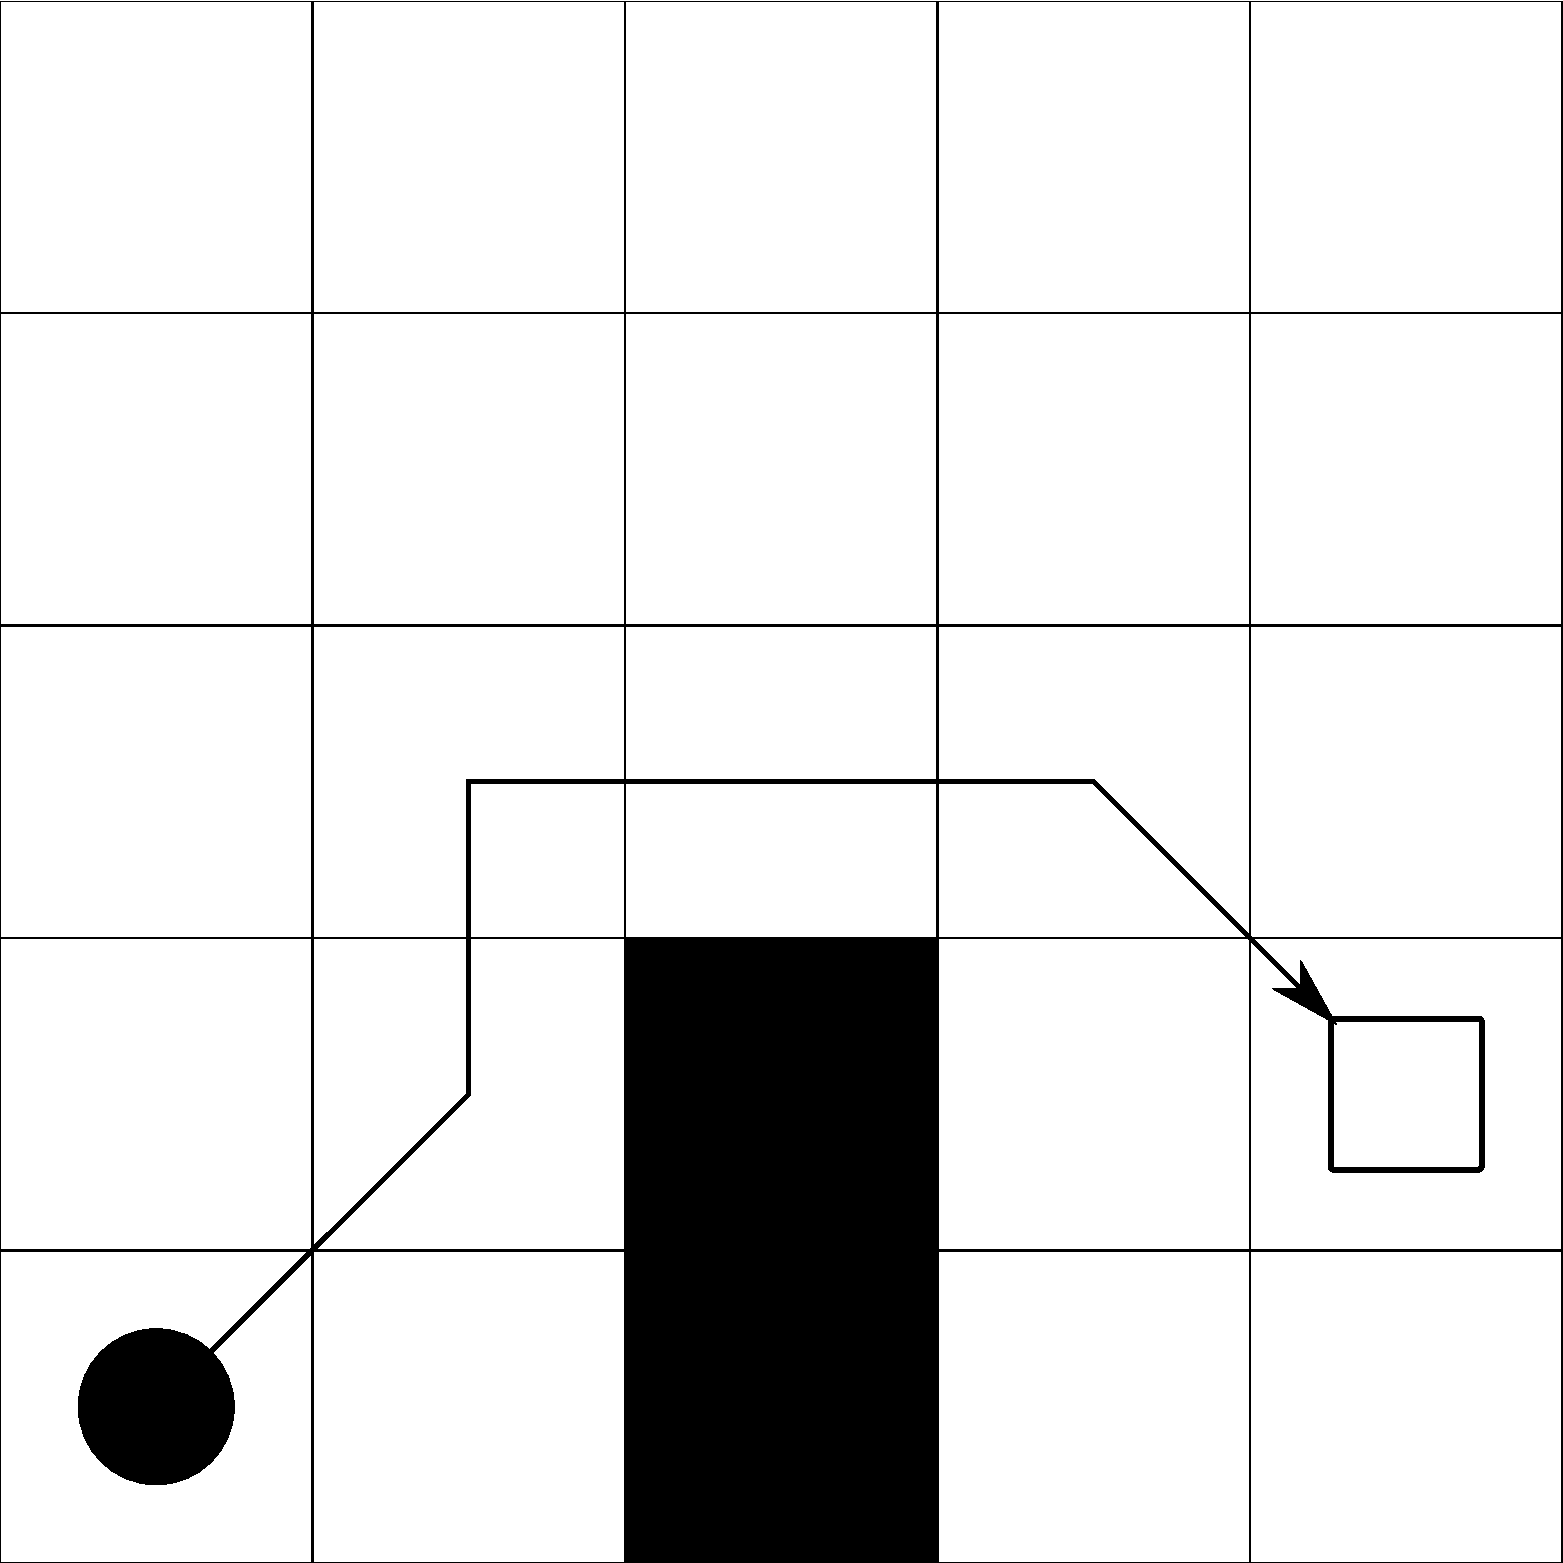
\includegraphics[width=0.3\linewidth]{images/basicGrid.pdf}
	\caption{}
	\label{fig:basicGrid}
\end{figure} 

Na slici~\ref{fig:basicGrid} prikazan je rezultat pretrage najkraćeg puta na ploči dimenzija \(5\times5\) na kojoj su mogući i dijagonalni prijelazi.
Ispunjeni krug predstavlja početnu poziciju, prazan kvadrat predstavlja cilj te ispunjeni kvadrati predstavljaju prepreke.
Neka se pločica u donjem lijevom kutu nalazi na poziciji \((1, 1)\), tada standardna formulacija problema slijedi u nastavku.
\begin{itemize}
    \item \(S\): sve pozicije od \((1, 1)\) i \((5, 5)\).
    \item \(S_0\): stanje \((1, 1)\).
    \item \(akcije(s)\): predstavlja prijelaze kojima se može doći do susjednih polja od \(s\) koji nisu prepreke. 
    Moguće vrijednosti su: \textit{gore}, \textit{dolje}, \textit{lijevo}, \textit{desno}, \textit{gore-lijevo}, \textit{dolje-lijevo}, \textit{gore-desno} i \textit{dolje-desno}. 
    Npr.\ za početno stanje \(S_0\) funkcija će vratiti slijed: \textit{gore}, \textit{desno} i \textit{gore-desno}. 
    \item \(prijelaz(s, a)\): funkcija vraća novu poziciju na polju kada se akcija \(a\) izvrši iz stanja \(s\). Npr. \(prijelaz((1, 2), gore)\) će vratiti stanje \((2, 2)\).
    \item \(cilj(s)\): funkcija je zadovoljena samo za \((5, 2)\).
    \item \(cijena(s, a)\): cijene prijelaza su Euklidove udaljenosti, odnosno prijelazi na strogo susjedna polja imaju cijenu \(1\), dok dijagonalni prijelazi imaju trošak \(\sqrt{2}\).
\end{itemize}

\par S obzirom na činjenicu da cijene prijelaza nisu uvijek iste, najbolje je odabrati algoritam pretrage koji uzima u obzir cijenu puta.
Najosnovniji takav algoritam pretrage je \textbf{pretraživanje s jednolikom cijenom} (engl. \textit{uniform-cost search}).

\par U isječku~\ref{fig:codeUCS} prikazan je pseudokod za algoritam pretraživanja s jednolikom cijenom. 
Algoritam inicijalizira početni čvor, prioritetni red sortiran po cijeni puta \(g(s)\) i skup posjećenih stanja. 
Prioritetni red je struktura u koju ubacujemo elemente koji se mogu sortirati po zadanom kriteriju i uvijek izvlačimo najveći ili (u ovom slučaju) najmanji element.
Algoritam zatim uvijek uzima čvor s najmanjom vrijednosti i provjerava ako je stanje u tom čvoru ciljno stanje.
Ako je uvjet ispunjen, algoritam vraća to rješenje.
U protivnom, čvor se dodaje u skup posjećenih stanja i dalje se proširuje, odnosno njegovi susjedi se dodaju u prioritetni red.
Bitno je naglasiti zadnji korak u proširivanju stanja, odnosno provjeri jeli čvor s istim stanjem već ubačen u prioritetni red ali s većim troškom.
U tom slučaju, potrebno je zamijeniti čvor u prioritetnom redu s novim čvorom.
Ovime osiguravamo da u trenutku kada se čvor izvuče iz prioritetnog reda, najkraći put do njegovog stanja je pronađen.

\vspace{3mm}
\begin{minipage}{\textwidth}
	\lstinputlisting[caption = {Pseudokod za pretraživanje s jednolikom cijenom},
    label={fig:codeUCS}]{codesnippets/ucs.txt}
\end{minipage}

\par Zbog navedenog svojstva, algoritam pretraživanja s jednolikom cijenom je \textbf{optimalan}, odnosno uvijek će pronaći optimalni put do odredišta ako ono postoji.

\par Unatoč tome što će algoritam uvijek pronaći najkraći put, ponekad će za to morati proširiti veliki broj stanja jer se u obzir uzima samo cijena puta, bez znanja da je taj čvor bliži cilju ili nije. 
Pretraživanje s jednolikom cijenom je dakle neusmjereni algoritam pretrage.

\subsection{Usmjerena pretraga}

\par Usmjereni algoritmi pretraživanja su algoritmi koji koriste heurističku informaciju kako bi se pretraživanje brže usmjerilo prema cilju.
U općenitom obliku ovakvog algoritma stanja se ubacuju u prioritetni red kao u pretraživanju s jednolikom cijenom, no umjesto da se koristi cijena puta \(g(s)\) koristi se \textbf{evaluacijska funkcija} \(f(s)\).

\par Odabir evaluacijske funkcije \(f\) definira strategiju pretrage. 
Funkcija \(f\) tipično ima kao komponentu \textbf{heurističku funkciju} \(h\), koja se definira kao procjena minimalnog troška puta od trenutnog čvora do cilja~\cite{book:AIModernApproach}.

\par Primjer takvog pretraživanje je pohlepno pretraživanje. 
Ono odabire onaj čvor koji se čini najbliži cilju, ne uzimajući u obzir trošak puta.
Evaluacijska funkcija \(f(s)\) se definira kao \(f(s) = h(s)\).

\par Poboljšanje tog algoritma je ujedno i najpoznatija implementacija usmjerene pretrage: \textbf{algoritam A*}. 
Kod njega se čvorovi vrednuju tako da se zbroji trošak puta \(g(s)\) i heuristika \(h(s)\):
\begin{equation}
f(s) = g(s) + h(s).
\end{equation} 

\par Prema tome, vrijednost \(f(s)\) predstavlja procjenu troška puta koji prolazi kroz stanje \(s\).
Ovaj algoritam je identičan pretraživanju s jednolikom cijenom, osim što se u prioritetni red za čvorove ubacuje vrijednost \(g(s) + h(s)\) umjesto \(g(s)\).

\subsubsection{Uvjeti za optimalnost algoritma A*}

\par Kako bi algoritam A* bio optimalan, heuristika mora zadovoljiti svojstvo \textbf{optimističnosti}.
Također je vrlo bitno svojstvo \textbf{konzistentnosti}.

\par Heuristika je optimistična ako nikad ne predvidi udaljenost do cilja koja je veća od stvarne. 
Kao posljedica činjenice da je \(g(s)\) cijena puta do stanja \(s\), \(f(s)\) nikad neće imati vrijednost veću od cijene stvarnog puta do cilja kroz čvor \(s\).
Matematički formulirano, ako je \(h^*(s)\) cijena stvarnog puta od čvora \(s\) do cilja, tada vrijedi:
\begin{equation}
\forall s \in S, h(s) \leq h^*(s).
\end{equation} 
Također, vrijednost heuristike u ciljnom čvoru mora biti 0: \(h(s_{cilj}) = 0\).

\par Heuristika je konzistentna ako procjena udaljenosti do cilja nikad nije veća od zbroja heurističke vrijednosti od susjednog stanja i cijene puta između navedena dva stanja.
Odnosno, ako je \(s\) trenutno stanje, \(s'\) susjedno stanje i \(a\) akcija koja vodi iz \(s\) u \(s'\), tada vrijedi:
\begin{equation}
h(s) \leq c(s, a) + h(s').
\end{equation} 
Ovo svojstvo je temeljeno na svojstvu nejednakosti trokuta, odnosno činjenici da zbroj duljina dviju stranica trokuta ne može biti manja od duljine treće stranice.
Analogija između to dvoje može se vidjeti na slici~\ref{fig:triangleInequality}.

\begin{figure}[h]
	\centering
	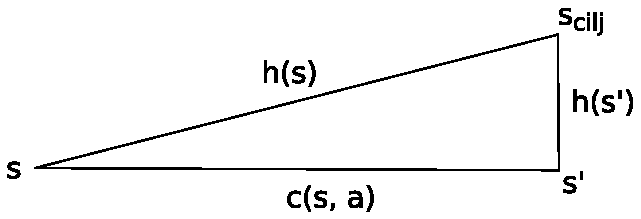
\includegraphics[width=0.5\linewidth]{images/triangleInequality.pdf}
	\caption{Veza između konzistentnosti heuristike i nejednakosti trokuta}
	\label{fig:triangleInequality}
\end{figure} 

\par Konzistentna heuristika je ujedno i optimistična, iako suprotno ne vrijedi. 
Samim time, konzistentnost je stroži uvjet od optimističnosti. 
U algoritmu A* konzistentnost heuristike osigurava da će se čvor proširiti kada je najkraći put do njega pronađen, poput pretraživanja s jednolikom cijenom.

\par Još jedno bitno svojstvo heuristike je \textbf{obaviještenost}. 
Jedan primjer heuristike koja zadovoljava uvjet optimističnosti i konzistentnosti je funkcija koja za svako stanje vraća 0: \(\forall S \in S, h(s) = 0\). 
Algoritam A* s ovakvom heuristikom degenerira pretraživanje s jednolikom cijenom, odnosno za svako stanje se gleda samo njegova cijena \(g\). 
Heuristika je bolja ako daje više informacija, odnosno ako funkcija \(h\) vraća veću vrijednost.

\section{Prilagodba na promjene}\label{sec:adaptation}

\par Likovi u računalnim igrama se moraju kretati glatko bez nepotrebnih stajanja, što znači da moraju pretraživati u realnom vremenu.
Nakon što se pretraga izvršiti, agent\footnote{objekt koji je izvršio pretragu} se mora fizički pomaknuti prema cilju.
U međuvremenu se na mapi mogu dogoditi razne promjene na koje se agent mora znati prilagoditi.

\par A* sam po sebi nije prikladan za taj posao, jer broj stanja koji se moraju pretražiti raste ovisno o ukupnom broju stanja. 
Također, A* ne zna prepoznati promjene u prostoru stanja, poput promjena na mapi. Kada bi se prilikom dolaska u svako novo stanje algoritam A* ponovo izvrtio, u najboljem slučaju jedinice bi u svakom novom stanju zastale dok se prostor pretraži te im kretanje ne bi više bilo glatko. 
U najgorem slučaju, čitava igra bila bi sklona čestim zaustavljanjima (engl. \textit{lag spike}).

\subsection{Ponovljeni A*}

\par Najjednostavnija modifikacija koja se može napraviti nad algoritmom A* kako bi bio iskoristiv u realnom vremenu je ograničenje pretrage na manji lokalni prostor.
Sva stanja u tom lokalnom prostoru također moraju biti u blizini agenta, odnosno udaljena samo određeni broj poteza.
Konkretno, postavi se ograničenje na broj stanja koji se mogu proširiti i ograničenje na broj poteza koje agent može napraviti.
Kada se izvrši pretraga iz trenutne pozicije, agent će krenuti prema stanju koje je trenutno sljedeće u prioritetnom redu sve dok ga ne dosegne ili dok ne napravi maksimalni broj dozvoljenih poteza.
Taj će se postupak ponavljati sve dok agent ne dostigne ciljni položaj.
Dodatno, može se definirati uvjet da ako se promjeni stanje koje se trenutno nalazi u trajektoriji (npr.\ ako se direktno na putu jedinici u RTS-igri izgradi zgrada), pretraga se ponovi s novim podatcima o okolini.

\par Zahvaljujući navedenim modifikacijama, algoritam A* se može koristiti u stvarnom vremenu. 
Broj posjećenih stanja bit će neovisan o broju mogućih stanja što garantira mali prostor stanja, no rezultirat će dužim putevima agenta do cilja.

\par S obzirom na činjenicu da svaka pretraga kreće ispočetka, moguća je pojava ciklusa. 

\begin{figure}[h]
	\centering
	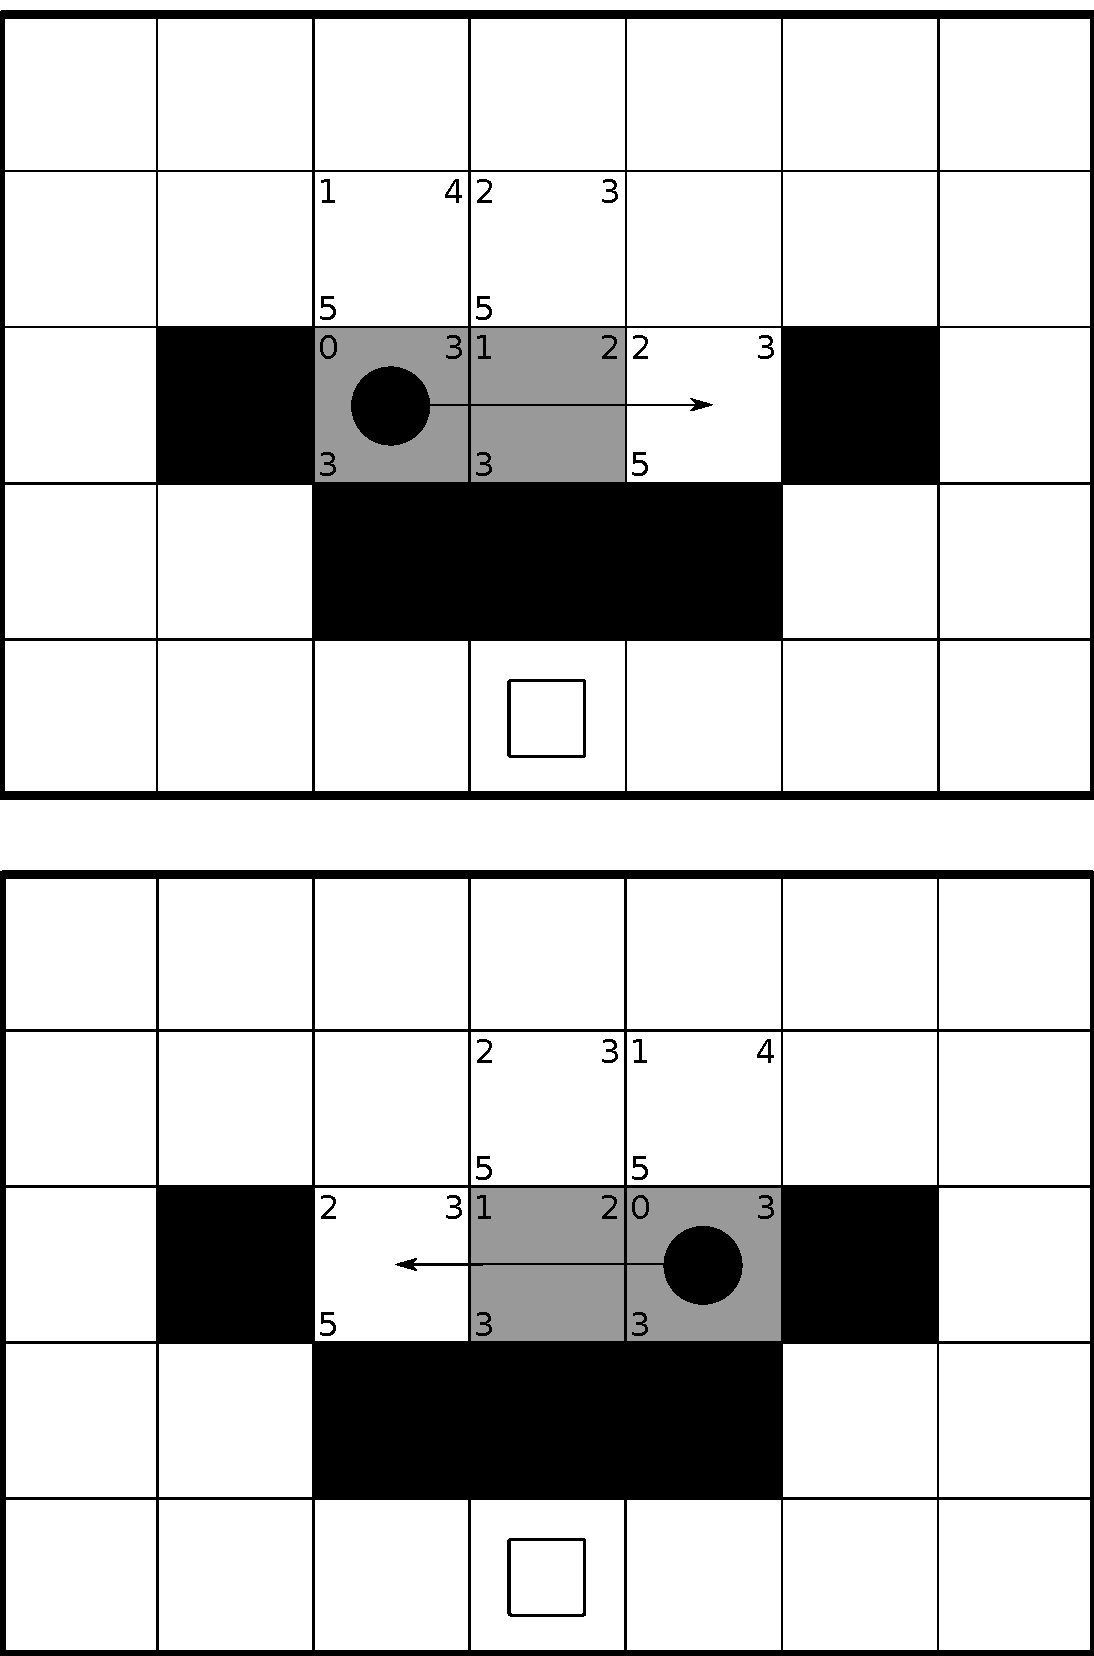
\includegraphics[width=0.45\linewidth]{images/repeatedAStarCycle.pdf}
	\caption{Pojava ciklusa kod ponovljene pretrage}
	\label{fig:pathfindingCycle}
\end{figure} 

\par Na slici~\ref{fig:pathfindingCycle} prikazan je rezultat pretrage koja je rezultirala ciklusom. 
Radi jednostavnosti, u ovom problemu dopušteni su samo pomaci na izravno susjedna polja.
Broj stanja koja se mogu proširiti ograničen na 2, te je agent zatim otišao prema idućem čvoru u prioritetom redu. 
Ispunjeni krug predstavlja početni položaj u pretrazi, kvadrat ciljni položaj, dok zasivljeno polje predstavlja pregledano stanje. 
U gornjem lijevom kutu zapisan je trošak puta za čvor \(g(n)\), u gornjem desnom kutu vrijednost heuristike \(h(n)\) te u donjem lijevom kutu vrijednost \(f(n) = g(n) + h(n)\).
U slučaju kada se u prioritetni red doda čvor s vrijednosti koja već postoji, prvi u redu je onaj koji je zadnji dodan.

\subsection{Adaptivni A* u stvarnom vremenu}\label{ssec:rtaastar}

\par Kako bi se riješio problem pojave ciklusa, potrebno je sačuvati informacije iz prijašnjih pretraga.
Jedan od algoritama koji nudi takvu mogućnost je adaptivni algoritam A* u stvarnom vremenu (engl. \textit{Real-Time Adaptive A*}, u nastavu RTAA*).

\par U praksi, često je potrebno izvesti više A* pretraga s konzistentnom heuristikom i istim ciljnim stanjem no s različitim početnim stanjima. Adaptivni algoritam A* će nakon svake pretrage podesiti heurističke vrijednosti posjećenih stanja kako bi buduće pretrage bile obavještenije~\cite{article:RTAAStar}.

\par Neka je \(s_{start}\) početno stanje u pretrazi i \(s\) stanje u lokalnom prostoru stanja. Ako je heuristika \(h\) konzistentna vrijedi relacija:
\begin{equation}
\forall s \in S, h(s_{start}) \leq g(s) + h(s).
\end{equation}
Drugim riječima, put od početne pozicije do cilja kroz stanje \(s\) nikad neće biti veće od stvarne udaljenosti od početnog stanja do cilja.

\par Ako je stanje \(\overline{s}\) prvo stanje u prioritetnom redu kada je lokalna pretraga završila, uvrštavanjem uvjeta konzistentnosti u gore navedenu formulu dobiva se sljedeći izračun:
\begin{equation}
\begin{aligned}
& \forall s \in S, f(\overline{s}) \leq g(s) + h(s)\\
& \forall s \in S, h(s) \geq f(\overline{s}) - g(s).
\end{aligned}
\end{equation}

\par Kao posljedica toga, za svako posjećeno stanje u pretrazi moguće je napraviti korekciju:
\begin{equation}
h(s) = f(\overline{s}) - g(s).
\end{equation}

\begin{minipage}{\textwidth}
	\lstinputlisting[caption = {Pseudokod za algoritam RTAA*~\cite{article:RTAAStar}},
    label={fig:codeRTAAStar}]{codesnippets/rtaastar.txt}
\end{minipage}

U programskom isječku~\ref{fig:codeRTAAStar} prikazan je pseudokod za algoritam RTAA*. 
Algoritam na početku obavi pretragu A* s maksimalnim brojem stanja za proširenje, te kao rezultat dobije stanje koje je bilo iduće i prioritetnom redu i skup posjećenih stanja.
Stanje koje je iduće bilo u prioritetnom redu postane trenutni cilj u kretanju agenta.
Ako pretraga A* nije vratila nikakvo rješenje znači da put do odredišta ne postoji, odnosno funkcija u tom slučaju vraća neuspjeh.
U suprotnom slučaju, prvo se napravi prilagodba heuristike za sva stanja u skupu posjećenih stanja.
Nakon toga, agent se počne kretati po mapi sve dok ne dostigne cilj ili ne obavi maksimalni broj pokreta.
U svakom novom stanju, agent provjerava sva stanja koja mu se nalaze na putanji do cilja.
Ako zabilježi promjenu bilo gdje na putu, znači da mu trenutna putanja potencijalno više nije valjana. 
U tom slučaju, petlja započinje ponovo izvođenjem pretrage A*.
Navedena petlja se ponavlja sve dok agent ne dostigne cilj ili ne shvati da put do istoga ne postoji.

\begin{figure}[h]
	\centering
	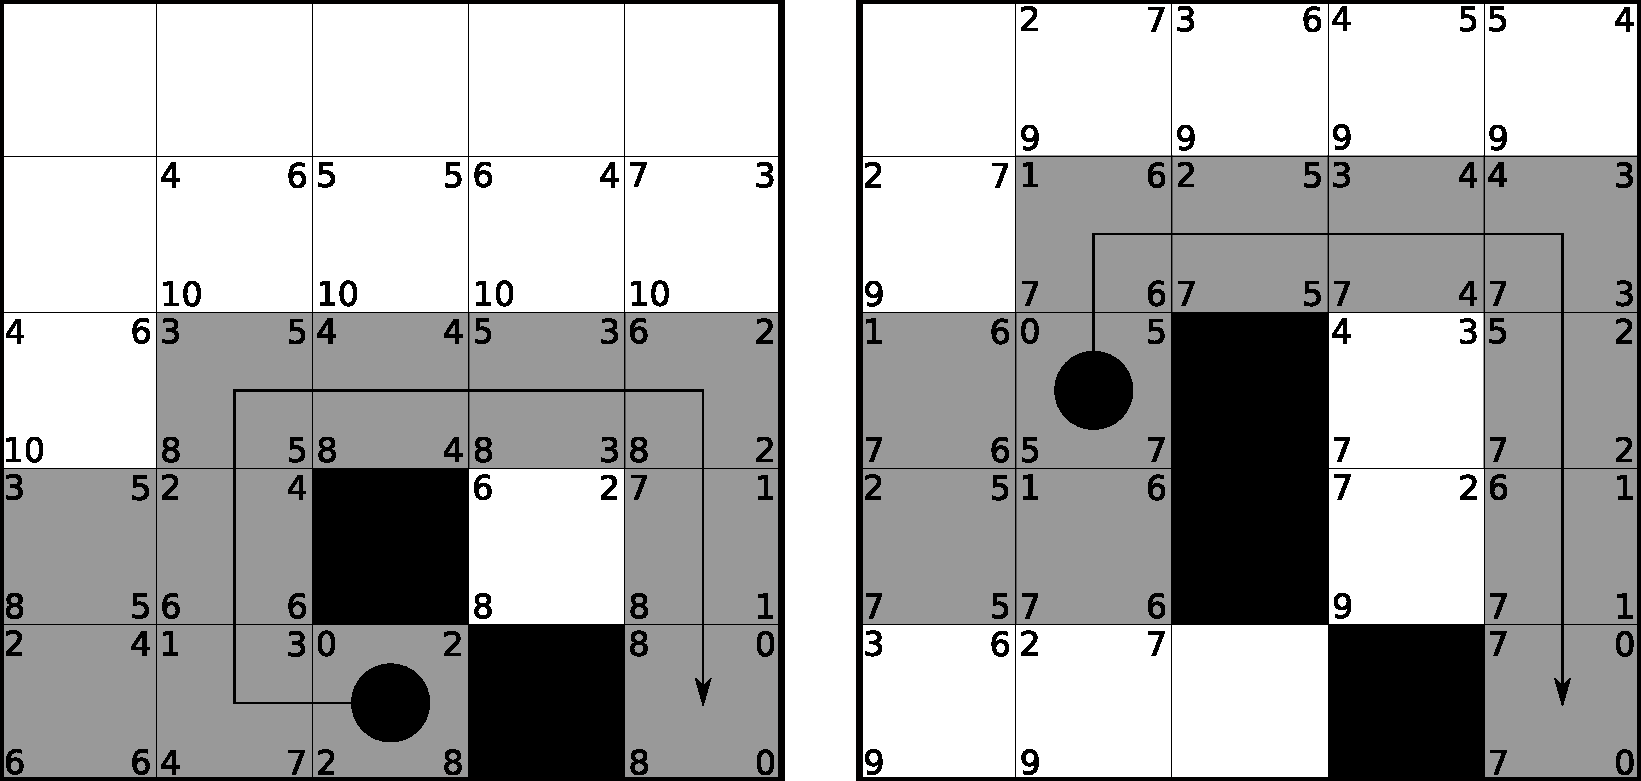
\includegraphics[width=0.9\linewidth]{images/rtaastar.pdf}
	\caption{Primjer pretrage RTAA*\cite{article:RTAAStar}}
	\label{fig:rtaastar}
\end{figure}

\par Na slici~\ref{fig:rtaastar} prikazan je primjer pretrage RTAA*.
Maksimalni broj pretraženih stanja u ovoj pretrazi nije ograničen, kao ni maksimalni broj poteza koje agent može napraviti.
Kao i s primjerom na slici~\ref{fig:pathfindingCycle}, u gornjem lijevog kutu prikazan je trošak \(g(s)\), u gornjem desnom \(h(s)\), u donjem lijevom \(f(s)\) te siva polja označavaju pretražena stanja.
Heuristička funkcija je definirana kao zbroj horizontalne i vertikalne udaljenosti do cilja, što je poznatije pod nazivom ''Manhattan heuristika''.

\par Nakon prve pretrage, agent se pomaknuo do pozicije \((2, 3)\) kada je na  terenu uočena iznenadna promjena: na poziciju \((3, 3)\) dodana je prepreka.
Kako se ta pozicija nalazi na putu do cilja, potrebno je ponoviti pretragu.
Prva pretraga ažurirala je vrijednosti heuristika \(h(n)\) za sva proširena stanja, što se vidi u donjem lijevom kutu ćelija.
U drugoj pretrazi te se vrijednosti gledaju kao heurističke vrijednosti za njihova stanja, što pretragu sprječava da se usmjeri prema prijašnjoj početnoj poziciji, odnosno \((3, 1)\).

\section{Grupiranje jedinica}\label{sec:grouping}

\par Algoritam A* i njegove inačice su sposobni pronaći put do cilja ali ne uzimaju u obzir taktičko pozicioniranje jedinica. 
Primjerice, ako igrač u RTS-igri odjednom odabere više od jedne jedinice i zada im odredište, očekivano ponašanje je da će se jedinice zajedno kretati kao skupina. 
Također, u borbi je poželjno da se jedinice nastoje pozicionirati na maksimalnoj udaljenosti od mete na kojoj i dalje mogu pucati, kao što se može vidjeti na slici~\ref{fig:enemySeparation}.

\begin{figure}[h]
	\centering
	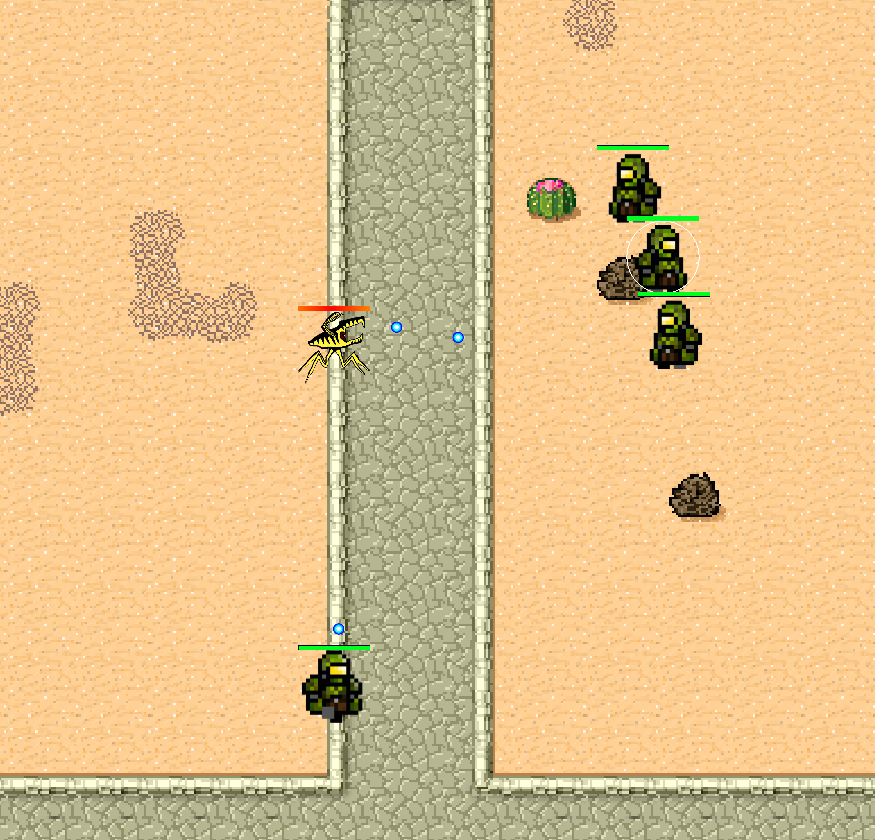
\includegraphics[width=0.5\linewidth]{images/enemySeparation.png}
	\caption{Pozicioniranje jedinica na maksimalnoj udaljenosti od mete}
	\label{fig:enemySeparation}
\end{figure}

\subsection{Algoritam \textit{Boids}}\label{ssec:boids}

\par Kada se jedinice grupiraju, njihovo kretanje prema cilju mora biti zajedničko.
Kada bi prilikom zadavanja cilja grupi jedinica za svaku jedinicu pokrenuli algoritam A*, one bi se kretale neovisno jedne o drugima. 
Zbog njihovih različitih pozicija, njihove putanje bi također mogle biti drastično različite. 
Također, ako se jedinice kreću po istim putanjama one će se često sudarati međusobno. 
Ovakav rezultat nije prihvatljiv s obzirom na očekivanje da će grupa jedinica biti jača i efikasnija od jedne same jedinice.

\par Inspiracija za implementaciju grupiranja jedinica dolazi iz prirode. 
Kretanje jata ptica ili java riba je sinkronizirano i fluidno iako se sastoji od kretanja mnogih individualnih životinja, gdje se ponašanje svake od njih temelji samo na njenoj lokalnoj percepciji svijeta.
Algoritam koji primjenjuje osnovne ideje ponašanja jata ptica i primjenjuje ih na ostale probleme zove se \textit{Boids}, što dolazi iz engl. \textit{bird-like objects}, odnosno \textit{birdoids}~\cite{article:FlocksHerdsSchools}.

\par Najosnovnija inačica algoritma \textit{Boids} sastoji se od tri pravila:
\begin{itemize}
	\item \textbf{odvojenost}: usmjeravanje jedinica kako bi se izbjegli sudari sa suborcima.
	\item \textbf{poravnatost}: usmjeravanje jedinica prema prosječnom smjeru kretanja grupe.
	\item \textbf{kohezija}: usmjeravanje jedinica prema centru mase grupe. 	 
\end{itemize}
Dodatna pravila se mogu dodati, poput zajedničkog kretanja prema trenutnom cilju, izbjegavanje sudara sa zgradama, izbjegavanje protivničkih jedinica, itd.

\par Algoritam \textit{Boids} ima razne ostale primjene, poput stabilizacije bespilotnih letjelica, izrade animacija te primjene u optimizacijskim problemima poput roja čestica (engl. \textit{Particle swarm optimization}).

\begin{figure}[h]
	\centering
	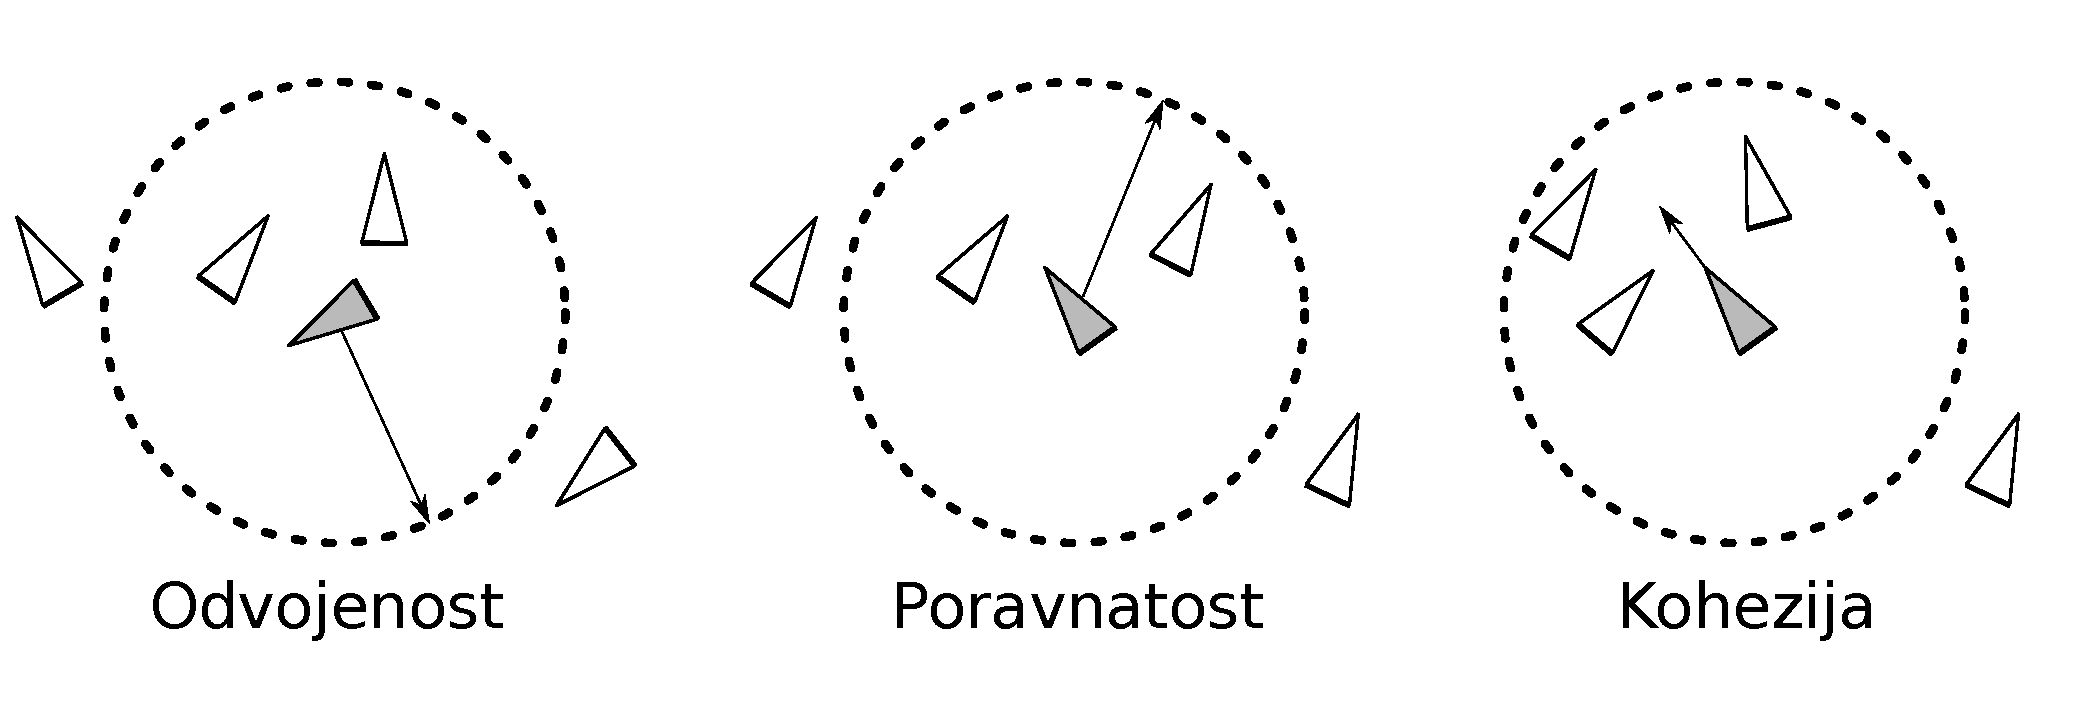
\includegraphics[width=1.0\linewidth]{images/boids.pdf}
	\caption{Tri osnovna pravila za algoritam \textit{Boids}}
	\label{fig:boids}
\end{figure}

\par Na slici~\ref{fig:boids} vizualizirana su navedena pravila odvojenosti, poravnatosti i kohezije. 
Sivi trokut predstavlja jedinicu nad kojom se navedene operacije trenutno obavljaju, dok iscrtani krug oko njega predstavlja radius u kojem se promatra ostale jedinice. 
Na crtežu za odvojenost na trenutni trokut djeluju dva trokuta iznad njega, što mu mijenja smjer prema smjeru označenim strelicom. 
U crtežu za poravnatost vektor smjera je okrenut prema smjeru prema kojem ostale jedinice putuju. 
U zadnjem crtežu vidi se primjer kohezije, odnosno smjer trenutnog trokuta se zakreće prema prosječnoj poziciji ostalih trokuta u radiusu.

\subsection{Hibridna navigacija}\label{ssec:hybrid}

\par Uz pomoć algoritma A* i algoritma \textit{Boids} postignuta je mogućnost kretanja skupine jedinica zajedno po mapi.
Sljedeća ideja je proširiti algoritam \textit{Boids} kako bi mogao rješavati problem taktičkog pozicioniranja jedinica u borbi.
Metoda navigacije u kojoj se jedinice kreću po mapi prema algoritmu A* dok nisu u blizini protivničkih jedinica i zgrada, a inače prevladava algoritam \textit{Boids}, naziva se hibridna navigacija (engl. \textit{hybrid pathfinding})~\cite{article:HybridPathdinding}.

\par Algoritam \textit{Boids} bit će modificiran tako da nastoji držati jedinice na maksimalnoj udaljenosti od neprijateljskih jedinica i zgrada na kojoj i dalje mogu pucati.
To se postiže tako da se u pravila za algoritam \textit{Boids} doda uvjet kada se protivnička meta pojavi unutar radijusa napada jedinice, njen vektor smjera se mijenja u smjeru suprotnom od protivničke pozicije.
Ako je riječ o jedinici s ograničenim ili nepostojećim borbenim sposobnostima poput radnika, njen cilj je držati se na udaljenosti većoj od protivničkog radijusa za napad.
Ovo se pravilo može proširiti i da vrijedi u slučaju da je borbena jedinica odlučno nadjačana, npr. ako jedna slaba jedinica naiđe na suparničku skupinu jačih jedinica.

\begin{figure}[h]
	\centering
	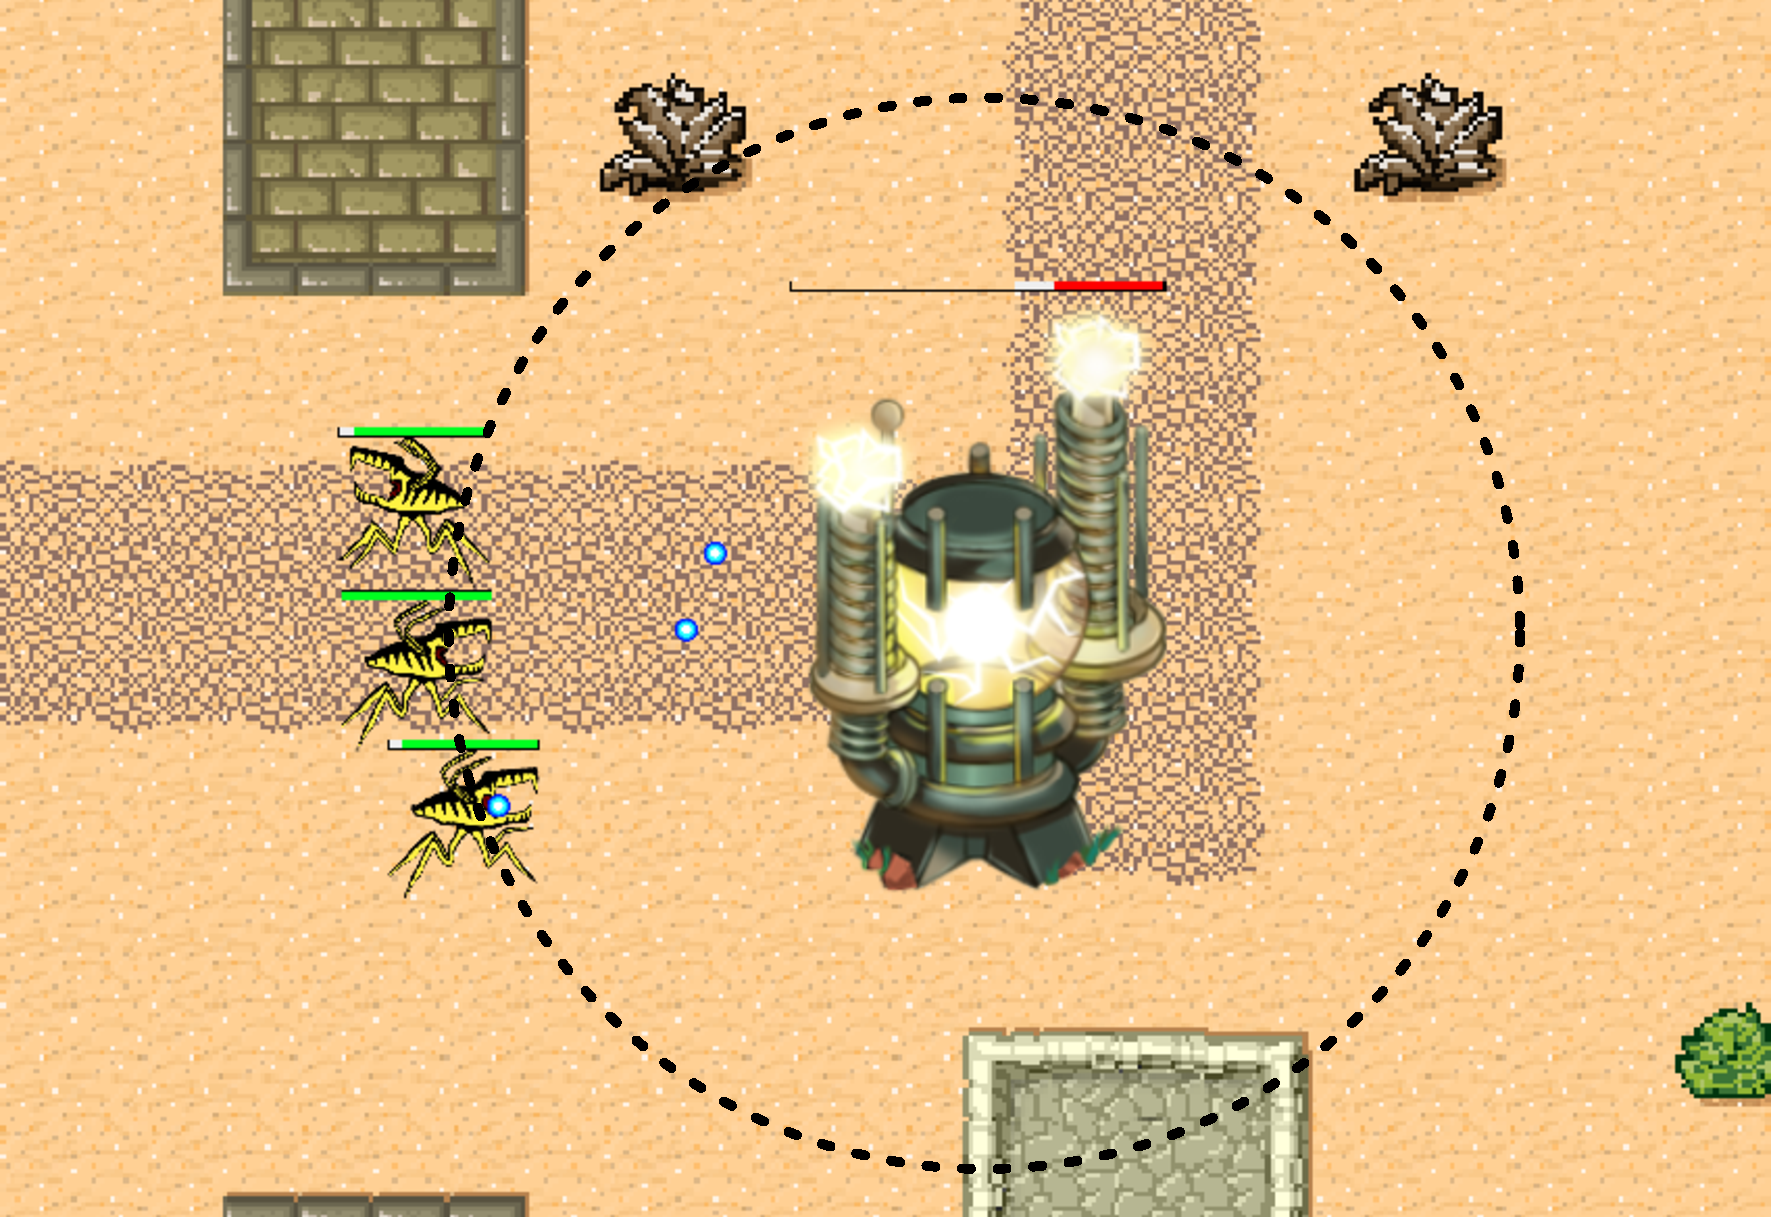
\includegraphics[width=0.8\linewidth]{images/boidsEnemySeparation.pdf}
	\caption{Odvajanje od protivničkih zgrada}
	\label{fig:boidsEnemySeparation}
\end{figure}

\par Na slici~\ref{fig:boidsEnemySeparation} prikazan je primjer u kojem su jedinice kojima upravlja bot\footnote{računalni program koji obavlja automatizirane poslove, poput upravljanja neprijateljskih jedinica protiv igrača} napale zgradu od ljudskog igrača.
Iscrtkanom kružnicom označena je maksimalna udaljenost s koje protivničke jedinice mogu pucati po igračevoj zgradi, te je vidljivo kako se protivničke jedinice drže te udaljenosti.

\chapter{Implementacija jezgrenih funkcionalnosti}\label{ch:implementation}

\par Programska implementacija napisana je u programskom jeziku Java, uz uporabu besplatne biblioteke otvorenog koda \textit{LibGDX}.
Biblioteka \textit{LibGDX} omogućava izradu mobilnih igara i igara za stolna računala koristeći istu bazu programskog koda. 
Za izradu i uređivanje mape korišten je besplatni uređivač mapa \textit{Tiled}.

\par Programska implementacija izdvojena je u tri glavna modula.
\begin{itemize}
	\item Modul \textit{pathfinding}: sadrži generalizirane strukture podataka i algoritme pretrage, te podsustav za kretanje jedinica.
	\item Modul \textit{genericRTS}: sadrži općenite funkcionalnosti RTS-igre, poput jedinica i zgrada.
	\item Modul \textit{core}: sadrži konkretan prototip RTS-igre napisane koristeći prijašnja dva modula.
\end{itemize}

\section{Izdvajanje jezgrenih funkcionalnosti}\label{sec:core}

\subsection{Objekti u igri}

\par U paketu \textit{hr.fer.zemris.zavrsni.rts.objects} iz modula \textit{genericRTS} nalazi se apstraktni razred \textit{AbstractGameObject} koji predstavlja sve objekte u igri.
U njemu se nalaze informacije o poziciji objekta, njegovoj veličini, vektoru kretanja, itd.

\par Iz njega se izvode 4 podrazreda bitna za općenitu funkcionalnost RTS-igre.
\begin{itemize}
	\item \textit{Building}: modelira zgradu koje se nalaze na mapi.
	\item \textit{Resource}: modelira izvor resursa na mapi.
	\item \textit{Projectile}: modelira projektil, poput metka, koji leti po mapi i vrši štetu nad metom koju pogodi.
	\item \textit{Unit}: modelira jedinicu, te sadrži implementaciju logike za samostalno kretanje jedinica. 
\end{itemize}
Također je prisutno sučelje \textit{ISquad} koje predstavlja grupu jedinica i njegove implementacije su zadužene za zajedničko kretanje jedinica.

\begin{figure}[h]
	\centering
	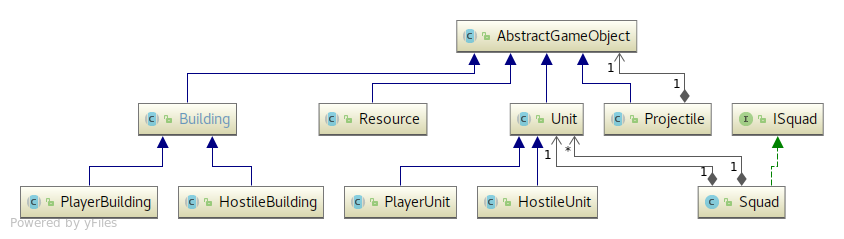
\includegraphics[width=0.8\linewidth]{images/umlObjects.png}
	\caption{Hijerarhija objekata u igri}
	\label{fig:umlObjects}
\end{figure}

\par Na slici~\ref{fig:umlObjects} vidljiva je opisana hijerarhija objekta.
Također su vidljivi tipovi \textit{PlayerUnit} i \textit{HostileUnit}, odnosno jedinice koje su na strani igrača i računala respektivno.
Isto to vrijedi i za tipove \textit{PlayerBuilding} i \textit{HostileBuilding}.
Dodatno, prikazan je tip \textit{Squad} koji implementira sučelje \textit{ISquad}.

\subsection{Uređivanje mape}

\par Alat za uređivanje mapa \textit{Tiled} nudi grafičko sučelje u kojem korisnik definira izgled terena i može pridijeliti dodatne podatke za lokacije, tipove terene ili mapu općenito.
Također nudi opciju izvoza izrađene mape u format \textit{TMX}\footnote{engl. \textit{Tiled map XML}}.
Uvoz i prikaz mapa u navedenom formatu je podržan unutar biblioteke \textit{LibGDX}.

\par Budući da je uređivanje mape implementirano uporabom alata \textit{Tiled} i formata \textit{TMX}, ovaj aspekt igre je većinom također neovisan o konkretnoj implementaciji.
Mapa se sama po sebi prikazuje kao niz pločica s teksturama na 2D plohi.
Taj dio dizajna mape može biti dijeljen između mnoštva igara iz različitih žanrova osim RTS-a.

\par Međutim, za bilo kakvu interakciju s mapom, potrebne su dodatne informacije.
Konkretno za RTS, kako bi jedinice pronašle najkraći put po mapi, igra mora pristupiti informaciji o tome gdje jedinica smije ili ne smije proći, na kojim mjestima se jedinica može kretati brže ili sporije, itd.
Primjerice, jedinica će se brže kretati po cesti nego po pijesku.
Jednostavni pristup za rješavanje tog problema je za svaku vrstu podloge na  terenu definirati modifikator brzine kretanja od 0 do 1.

\begin{figure}[h]
	\centering
	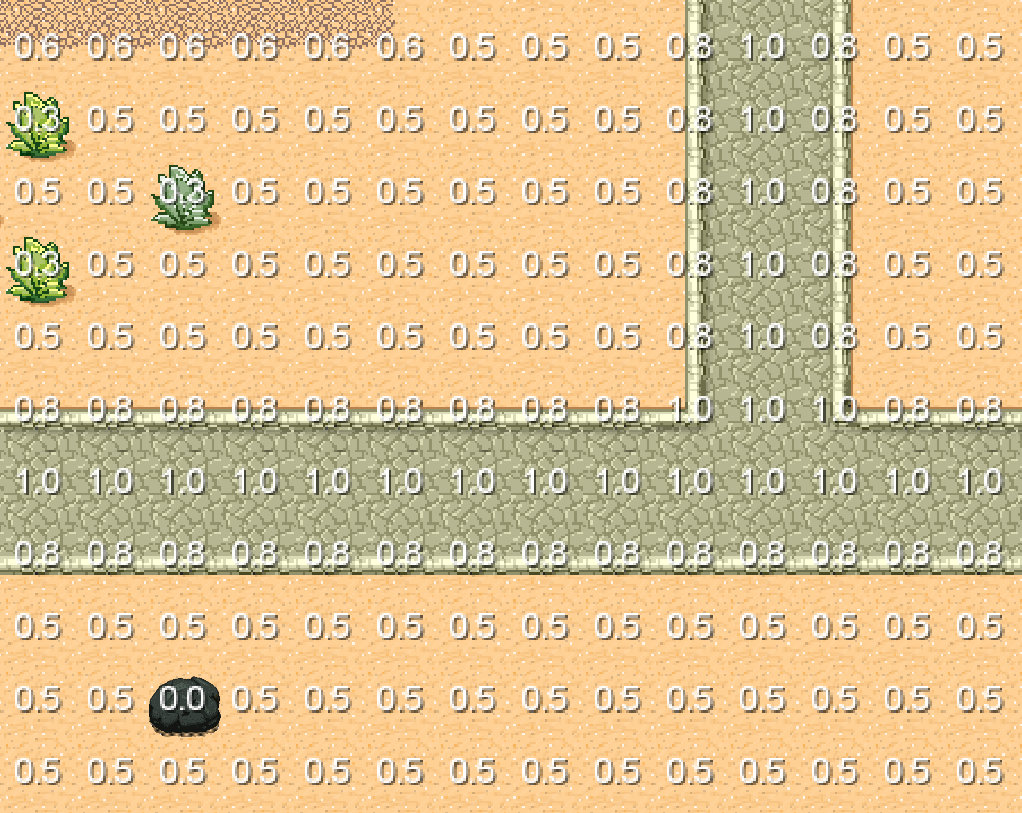
\includegraphics[width=0.6\linewidth]{images/tileModifiers.png}
	\caption{Prikaz modifikatora kretanja na mapi}
	\label{fig:tileModifiers}
\end{figure}

\par Na slici~\ref{fig:tileModifiers} prikazan je primjer gdje svaka pločica na mapi ima definiran modifikator brzine kretanja ovisno o svojem materijalu.
Žućkasta dio terena predstavlja pijesak, dok siva kamena tekstura predstavlja cestu.
Kao što se vidi, na cesti je modifikator kretanja \(1.0\) dok je na samom pijesku brzina kretanja dvostruko manje, odnosno \(0.5\).
Također, u gornjem lijevom kutu prikazani su grmovi kroz koje se jedinica može još sporije kretati, uz modifikator \(0.2\).

\par Konačno, zadnji skup podataka koji mora biti zapisan u opisu mape su položaji konkretnih resursa, zgrada i jedinica.
Oblik ovog zapisa ovisi o konkretnoj implementaciji igre te se može zapisati na razne načine.
Jedan pristup za riješiti taj problem je da se u alat za uređivanje mapa dodaju objekti koji će svi imati ključ koji definira o kojem se tipu objekta  iz RTS-igre radi.
Primjerice, mapa će imati objekt s ključem \textit{rock} koji predstavlja stijenu.
Tijekom učitavanja mape u igru, za svaki objekt s ključem \textit{rock} bit će kreirani izvor resursa na odgovarajućoj lokaciji.

\subsection{Kretanje jedinica}

\par U modulu \textit{pathfinding} nalaze se strukture podataka za izvršenje pretrage prostora stanja.
Primjerice, sučelje \textit{ISearchProblem} definira problem pretrage, odnosno početno stanje, provjeru krajnjeg stana i izračun idućih stanja i akcija. 
Također su definirana sučelja \textit{IHeuristic} koji definira funkciju heuristike i \textit{ISearchAlgorithm} koji definira algoritam pretrage nad problemom s definiranom heuristikom.

\par Osim općenitih sučelja, u ovom modulu nalaze se i osnovne implementacije te logike za navigaciju po 2D-mapi s mogućnosti dijagonalnih poteza.
Uz osnovne algoritme, tu se također nalazi implementacija algoritma RTAA* opisanog u potpoglavlju~\ref{ssec:rtaastar}.

\section{Implementacija protipa RTS-igre}

\par Uz opisanu jezgrenu funkcionalnost RTS-igre, izrađen je prototip jedne konkretne igre koja sadrži opisane osnovne funkcionalnosti.

\subsection{Pravila igre}

\par U navedenoj igri igrač započinje igru s bazom i jednim robotskim radnikom.
Na mapi nalaze se minerali koje radnik može skupljati.
Sa skupljenim mineralima moguće je izgraditi nove radnike, vojnike i toranj koji automatski puca na neprijatelje.

\par Na mapi se također nalaze protivničke baze i jedinice.
Protivničke baze će tijekom otprilike svakih 10 sekundi stvoriti novu protivničku jedinicu.
Kada baza stvori tri jedinice, one se grupiraju i kreću u napad na igračevu bazu.
Da bi se stigao pripremiti, igrač se mora čim prije moć obraniti te nakon toga krenuti u napad.

\par Jedinice iz suparničkih strana će se same početi međusobno boriti čim dođu međusobno u domet.
Također, igračeve jedinice će automatski početi pucati na protivničku bazu čim se ona nađe u dometu.
Tvrdnja vrijedi i za protivničke jedinice kada im se u dometu nađe igračeva baza.

\par Cilj u igri je uništiti sve protivničke baze i jedinice bez da igrač izgubi svoju.

\subsection{Prikaz funkcionalnosti igre}

\par Jedinice se u igri odabiru tako da igrač povuče lijevi klik miša, što se vizualizira pravokutnikom koji predstavlja označeno područje, čime se označavaju sve jedinice unutar tog pravokutnika.
Igrač zatim zadaje naredbe jedinicama koje su trenutno označene tako da klikne na proizvoljnu poziciju na mapi desnim klikom miša.
Označene jedinice će se zatim grupirati ako su dovoljno blizu i krenuti zajedno prema cilju.

\begin{figure}[h]
	\centering
	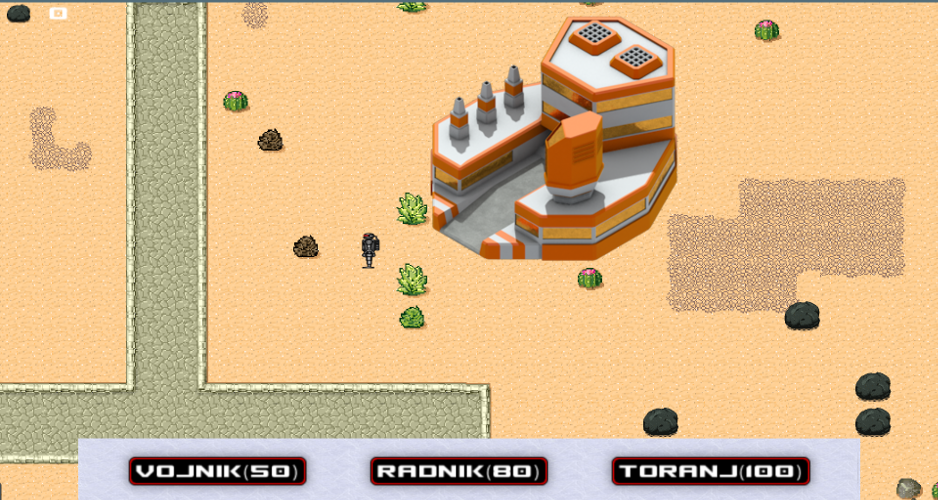
\includegraphics[width=0.9\linewidth]{images/gameStart.png}
	\caption{Početno stanje u igri}
	\label{fig:gameStart}
\end{figure}

\par Na slici~\ref{fig:gameStart} prikazano je početno stanje pri pokretanju nove igre.
Narančasta zgrada predstavlja igračevu bazu, te se lijevo od nje nalazi robotski radnik.
Crne stijene desno ispod baze predstavljaju izvore minerala.
Ikona minerala u gornjem lijevom kutu s brojkom 0 pored nje predstavlja količinu skupljenih minerala koji dosad nisu potrošeni.
Na dnu ekrana se također nalazi izbornik iz kojeg igrač bira na što želi trošiti resurse, te je u zagradama napisana cijena prikazanog izbora, te crveni obrub oko tipke označava nemogućnost odabira zbog manjka resursa.

\begin{figure}[h]
	\centering
	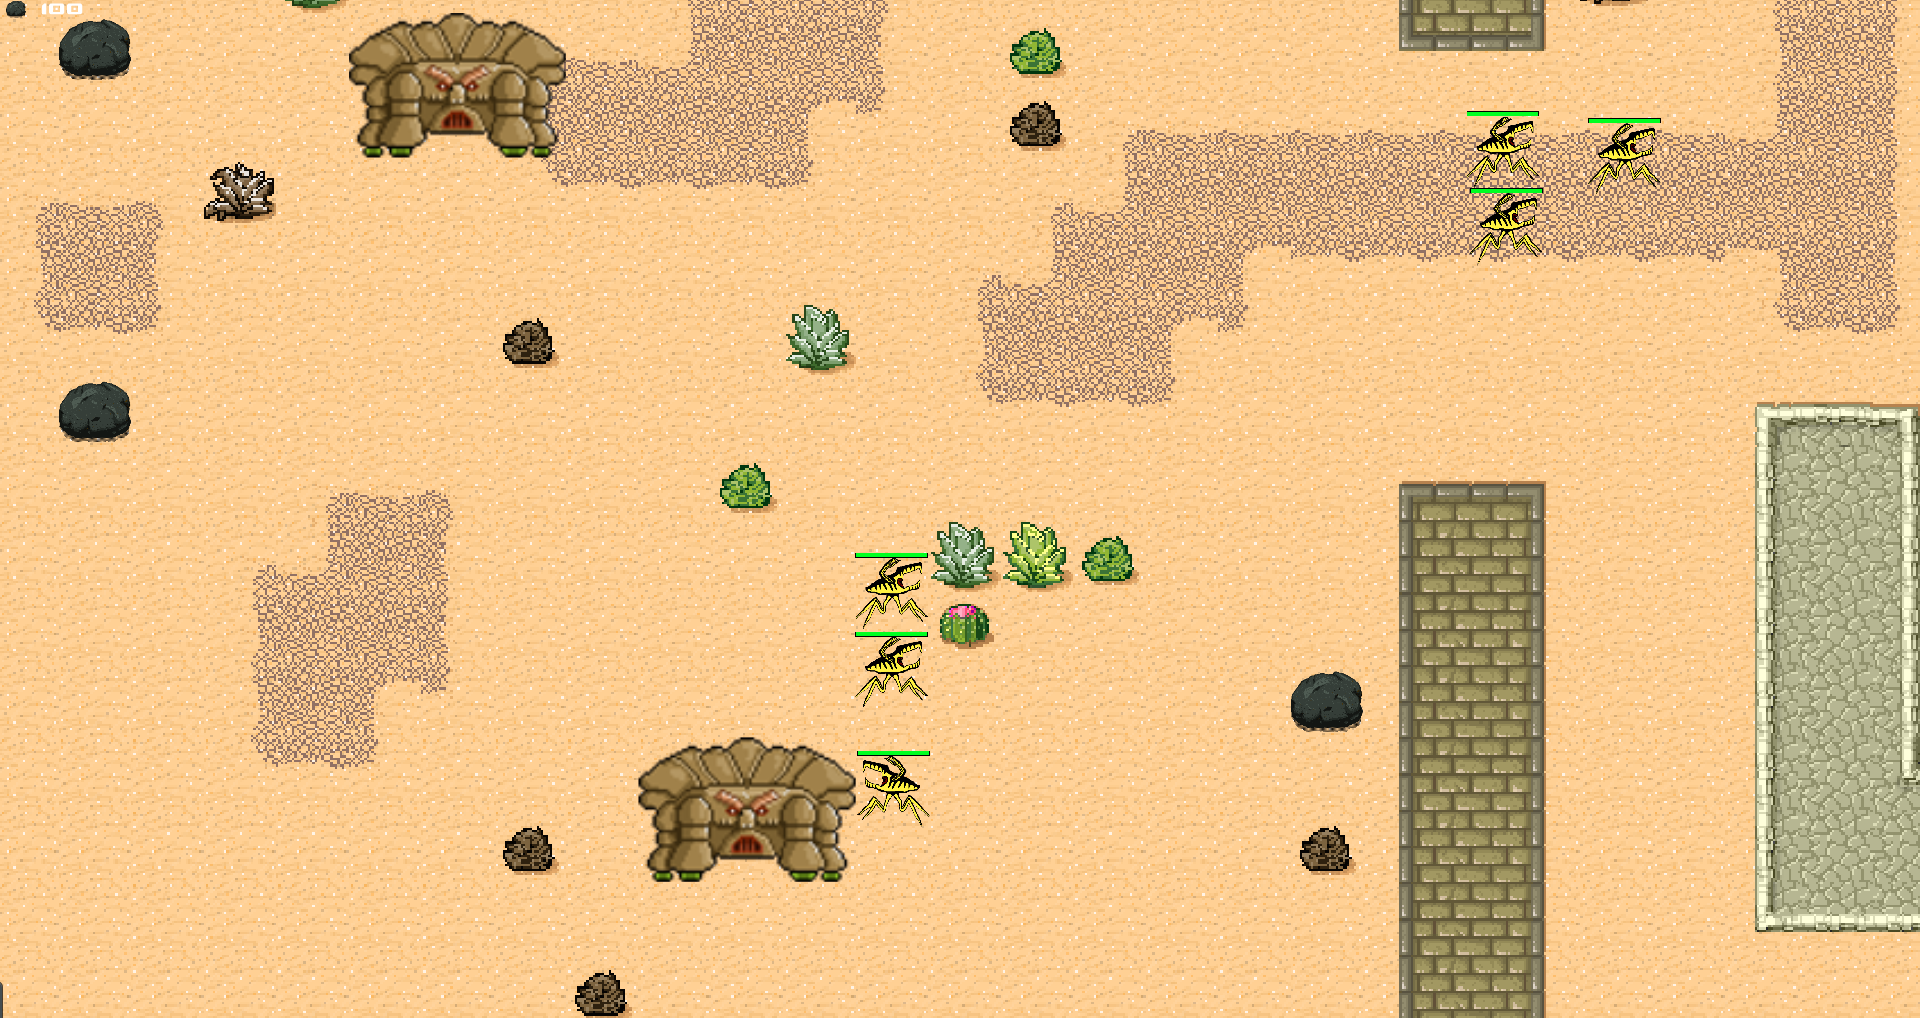
\includegraphics[width=0.9\linewidth]{images/enemyBases.png}
	\caption{Neprijateljske baze u igri}
	\label{fig:enemyBases}
\end{figure}

\par Na slici~\ref{fig:enemyBases} prikazane su neprijateljske baze i dvije skupine od tri jedinica koje kreću u napad na igračevu bazu.

\par Borba započinje kada se igračeva jedinica nađe u dometu protivničke jedinice, ili suprotno.
Protivničke jedinice koriste hibridnu navigaciju opisanu u potpoglavlju~\ref{ssec:hybrid}, odnosno nastoje se držati na maksimalnoj udaljenosti od igračevih jedinica na kojoj mogu i dalje pucati, najčešće formirajući polukrug oko navedene mete.

\begin{figure}[h]
	\centering
	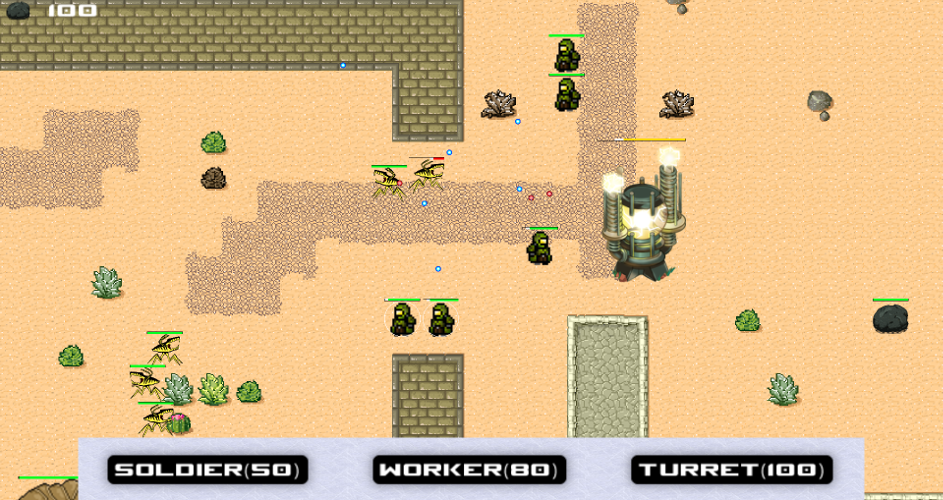
\includegraphics[width=0.9\linewidth]{images/battle.png}
	\caption{Prikaz borbe u igri}
	\label{fig:battle}
\end{figure}

\par Na slici~\ref{fig:battle} prikazan je primjer borbe u igri.
Pet igračevih vojnika bore se protiv dviju protivničkih jedinica te im u bitci pomaže defenzivni toranj koji također puca na protivnike.
Iz lijevog donjeg kuta se približava idući val neprijateljskih jedinica.
Iznad svake jedinice i zgrade nalazi se crta koja označava njihovo trenutno ''zdravlje''.
Puna zelena crta označava da jedinica ili zgrada nije ozlijeđena, dok crvena skoro prazna crta znači da je jedinica pred smrti.
Također je vidljivo da igračeve jedinice pucaju plave metke, dok protivničke jedinice pucaju crvene.

\par Resursi u igri se skupljaju tako da igrač odabere radnika i naredi mu da se skuplja određeni izvor resursa, odnosno izvor minerala.
Naredba za skupljanje se zadaje tako da se stijena klikne desnim klikom miša dok je neki radnik izabran.
Taj će radnik zatim pronaći put do navedenog resursa i početi ga skupljati kada mu dođe u blizinu.
Nakon što se resurs skupi, odgovarajuća količina minerala bit će dodana igraču.
Također, ako u blizini postoje ostali izvori materijala, radnik će ih samoinicijativno krenuti skupljati.
Bez ove mogućnosti, radnici bi zahtijevali previše mikroupravljanja te bi igrač redovito morao skretati pozornost s bitke samo kako bi zadao jednostavnu naredbu radniku.

\par Kada je skupljeno dovoljno minerala za izgraditi zgradu, igrač može klikom na gumb \textit{Toranj (100)} izabrati da želi izgraditi navedenu zgradu.
Time će se pojaviti silueta zgrade koja prati lokaciju koju miš označuje na mapi, kao što je prikazano na slici~\ref{fig:building}.
Korisnikovim klikom na lokaciju na mapi će zgrada biti izgrađena na tom mjestu, ako je moguće.
Ako korisnik označi lokaciju na kojoj se zgrada ne može izgraditi, ili ako za izgradnju zgrade nisu dostupni resursi, silueta zgrade će biti crvena.

\begin{figure}[h]
	\centering
	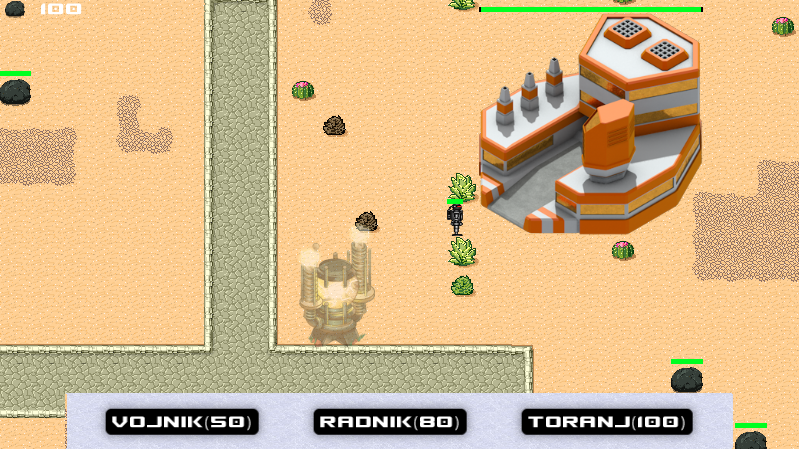
\includegraphics[width=0.9\linewidth]{images/building.png}
	\caption{Izgradnja novih zgrada u igri}
	\label{fig:building}
\end{figure}

\par Tijekom igre igrač ima mogućnost spremanja stanja trenutne igre na disk.
Ta ista igra se zatim može učitati i nastaviti bilo kada, odabirom prikladne mogućnosti u početnom ekranu.

\par Na slici~\ref{fig:menus} prikazani su izbornici dostupni u igri.
Gornja lijeva slika prikazuje početni izbornik koji nudi opciju pokretanja nove igre, učitavanja stare, ulaska u postavke i izlaska iz igre.
U gornjoj desnoj slici prikazan je izbornik koji se pojavi kada igrač pritisne tipku za povratak unutar igre.
Omogućuje igraču povratak u igru, spremanje igre na disk, ulazak u postavke i povratak na početni izbornik.
Donja slika prikazuje izbornik s postavkama.
U njemu su omogućene sljedeće mogućnosti.
\begin{itemize}
	\item Prikaz brojača slika u sekundi (engl. \textit{Frames per second}, FPS).
	\item Prikaz trenutno planiranih putanja jedinica.
	\item Prikaz indikatora \textit{zdravlja} igračevih jedinica.
	\item Prikaz indikatora \textit{zdravlja} protivničkih jedinica.
	\item Prikaz indikatora \textit{zdravlja} izvora resursa na mapi.
	\item Prikaz indikatora \textit{zdravlja} zgrada.
	\item Odabir jezika za igru. Podržani su engleski i hrvatski.
\end{itemize}

\begin{figure}[h]
	\centering
	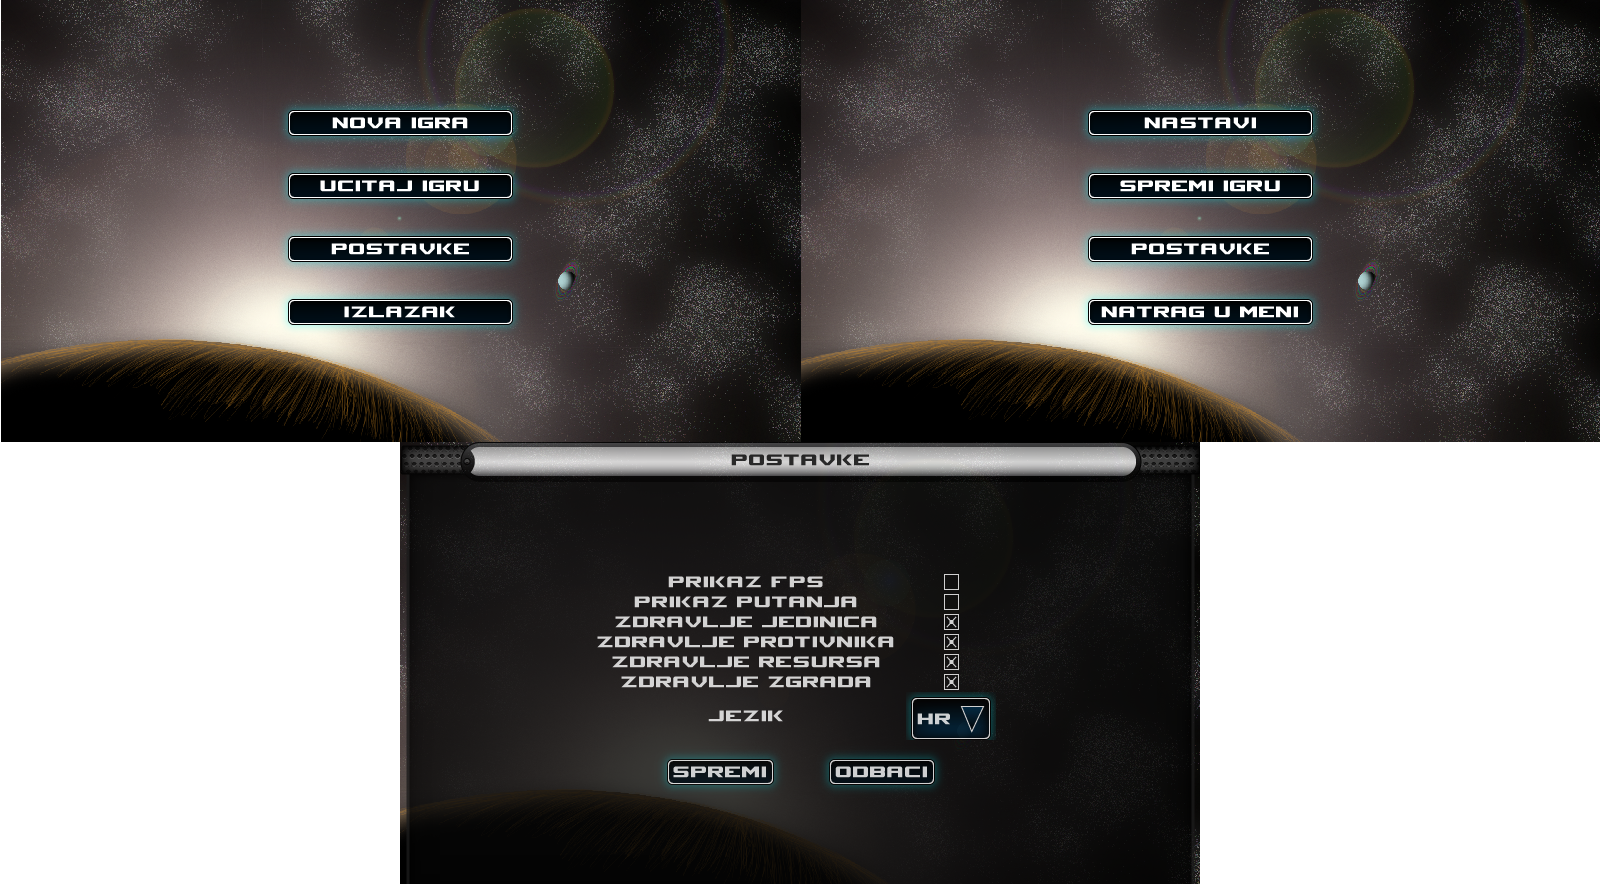
\includegraphics[width=1.0\linewidth]{images/menus.png}
	\caption{Prikaz izbornika u igri}
	\label{fig:menus}
\end{figure}

\section{Dodavanje novih funkcionalnosti}

\par Jedna od ključnih ideja tijekom razvoja jezgrenih funkcionalnosti RTS-igre bila je jednostavno proširivost igre.
U ovom potpoglavlju bit će prikazano nekoliko primjera kako se mogu jednostavno dodati nove zgrade i jedinice u prethodno opisanu igru.

\par Bitno je napomenuti da se za sve dodane objekte u igru moraju definirati teksture s kojima će se objekti prikazivati.
Novi objekti dodani u ovom poglavlju su osnovne slike izrađene u besplatnom alatu za uređivanje alata \textit{GIMP}.

\vspace{3mm}
\begin{minipage}{\textwidth}
	\lstinputlisting[caption = {Isječak koda u Javi koji dodaje novu protivničku jedinicu},
    label={fig:codeStickman}, language=Java]{codesnippets/stickman.java}
\end{minipage}\

\par U programskom isječku~\ref{fig:codeStickman} prikazan je programski isječak za dodavanje nove jedinice.
Tekstura kojom će se jedinica prikazivati spremljena već je izrađena i učitana u jedinstvenom objektu \textit{Assets}, kojem se pristupa iz metode \textit{loadAnimation()}.
Tijekom nasljeđivanja razreda \textit{HostileUnit}, potrebno je definirati sve atribute koji mogu biti različiti za svaku jedinicu.
Ova konkretna jedinica ima natprosječnu brzinu kretanja i brzinu napada, no ima nisko zdravlje i moć napada.

\par Ovaj je razred također implementirao sučelje \textit{IBuildableUnit}, što definira metodu \textit{getTrainingCost}.
Ovo daje informaciju igri o utrošku rada koji je potreban da se jedinica ovog tipa izgradi.
Primjer tog rada je kada igrač da naredbu da se izgradi vojnik, igračeva baza će obaviti količinu rada koja je definirana u navedenoj metodi za vojnika.

\par Uz pretpostavku da tekstura za ovu jedinicu uspješno napravljena, navedeni isječak koda je dovoljan da ona bude funkcionalna unutar igre.
Nažalost, s obzirom na činjenicu da je u prijašnjem isječku dodana samo definicija jedinice, ostatak igre ne zna za nju zbog čega se ona ne može prirodno pojaviti u igri.

\par Taj problem će se riješiti dodavanjem novog tipa zgrade.
Sve što treba napraviti je naslijediti razred \textit{HostileBuilding} i implementirati logiku kojom će ta zgrada stvarati primjerke jedinica \textit{Stickman}, kao što je prikazano u programskom isječku~\ref{fig:codeStickmanSpawner}.

\vspace{3mm}
\begin{minipage}{\textwidth}
	\lstinputlisting[caption = {Isječak koda u Javi koji dodaje novu zgradu},
    label={fig:codeStickmanSpawner}, language=Java]{codesnippets/stickmanSpawner.java}
\end{minipage}\

\par U navedenom isječku nadjačana je metoda \textit{update} koja se pozove u svakoj iteraciji glavne petlje igre.
U svakom pozivu metode \textit{update} obavlja se određeni rad prema stvaranju nove jedinice, koja se zatim dodaje u igru pozivom metode \textit{spawnUnit}.

\par Sada je nova zgrada spremna da bude funkcionalna unutar igre tako što može stvarati primjerke jedinica tipa \textit{Stickman}, što je vidljivo na slici~\ref{fig:stickman}.

\begin{figure}[h]
	\centering
	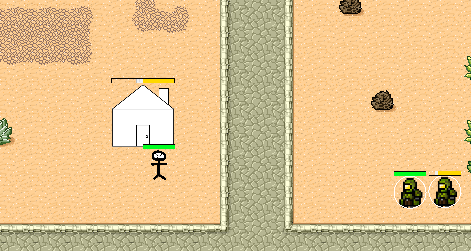
\includegraphics[width=0.7\linewidth]{images/stickman.png}
	\caption{Implementacija dodatnih funckionalnosti u igri}
	\label{fig:stickman}
\end{figure}

\par Definirani postupak dodavanja osigurava da nove zgrade i jedinice nisu ovisne o konkretnoj implementaciji ijedne RTS-igre.
Bilo koja RTS-igra koja koristi opisani podsustav može slobodno koristiti objekte \textit{Stickman} i \textit{StickmanSpawner}.

\par Isti taj postupak je analogan i za dodavanje novih izvora resursa.
Komplikacija s dodavanjem novih izvora resursa nastaje zato što svaki izvor mora definirati koji će resurs dodati igraču kada se uništi.
U ovom podsustavu, resurs prilikom uništenja pošalje igri odgovarajuću količinu resursa i ključ koji ga definira.
Zahvaljujući tome, bilo koja konkretna implementacija RTS-igre koja koristi minerale kao resurs može koristiti bilo koje izvore minerala, dokle god je dogovoreni isti ključ.
U prikazanoj konkretnoj implementaciji minerali su označeni ključem \textit{minerals}.

\chapter{Zaključak}\label{ch:conclusion}

\par U radu su proučeni i implementirani osnovni podsustavi RTS-igre.
Ti su podsustavi napisani kao vanjska biblioteka koja se može koristiti za razvoj konkretne RTS-igre.
Time je korisniku biblioteke omogućen jednostavniji razvoj igre, budući da su podsustavi za prikaz mape te kretanje i ponašanje jedinica već napisani i ponovo iskoristivi.

\par Kretanje jedinica svodi se na pretraživanje prostora stanja u kojem stanja predstavljaju pozicije na mapi.
Na većim mapama, prostor stanja će također biti veći.
Algoritam RTAA* omogućava da se veliki prostori stanja pretraže bez porasta složenosti, što ga čini prikladnim za pretragu u stvarnom vremenu.

\par Algoritam \textit{Boids} omogućio je zajedničko kretanje jedinica te osnovno ponašanje protivničkih jedinica.

\par Navedeni algoritmi su u konkretnoj implementaciji ostvarili vrlo dobre rezultate.
Grupirane jedinice su se zajednički kretale prema cilju uz sposobnost izbjegavanja prepreka i prilagodbe na promjene.

\par U konkretnoj igri implementirano samo osnovno ponašanje protivničkih jedinica. Zanimljivi izazov za daljnji razvoj bila bi umjetna inteligencija sposobna pametno igrati protiv ljudskog igrača.
Takav bi sustav morao donositi odluke na razini makro-upravljanja, odnosno pratiti stanje igre, inteligentno upravljati jedinicama, skupljati resurse i prikladno ih trošiti. 

\bibliography{literatura}
\bibliographystyle{fer}

\begin{sazetak}
Računalne igre značajan pokretač razvoja računala. 
Postoji mnoštvo vrsta računalnih igara, a posebno  interesantne vrsta igara čine strategije u stvarnom vremenu (engl. Real-Time Strategy, RTS). 
Razvoj takvih igara općenito uključuje pisanje mnogih podsustava i razvoj funkcionalnosti koje nisu specifične za konkretnu  igru pa ih je moguće višestruko iskorištavati.  
Takve funkcionalnosti  moguće je izolirati u zaseban razvojni okvir.
U okviru završnog rada razmatrani su elementi prisutni u RTS-igri, uz  programsku implementaciju osnovnih podsustava koje su moguće za dijeljenje između različitih RTS-igara. 
Oživotvoren je prototip jedne konkretne igre koja sadrži osnovne elemente poput prikaza mape svijeta, stvaranja građevina različitih  funkcija (proizvodnja, obrana) te jedinica, upravljanje jedinicama (grupiranje, zadavanje ciljeva:  dolazak na zadani položaj, pucanje, prikupljanje resursa) i osnovno upravljanje protivničkim jedinicama. 
Implementaciju je ostvarena u programskom jeziku Java. 
Rad sadrži algoritme, izvorne kodove i rezultate uz potrebna objašnjenja i dokumentaciju.

\kljucnerijeci{RTS, navigacija, A*, \textit{Boids}, \textit{LibGDX}, Java }
\end{sazetak}

\engtitle{Implementation of RTS game core}
\begin{abstract}
Computer games represent a significant catalyst in the development of computers.  
There are many genres of computer games whereby Real-Time Strategy games represent one of the more interesting genres. 
The development of those types of games generally involve developing  a variety of subsystems and functionalities which are not specific for a particular game, and are thus suitable for multiple use. 
These functionalities can be isolated into a separate workspace.   
This thesis reviews the elements present in an RTS game and develops a program implementation of the basic subsystems that can be shared between various RTS games. 
A prototype of a particular game was developed containing basic elements, such as the rendering of the world map, the construction  of buildings serving various functions (industry, defence) as well as units, the management of units (grouping, assigning objectives: arrival to the defined location, shooting, resource gathering)  and the basic management of enemy units. 
The implementation was written in the Java programming language. 
The theses includes the algorithms, source code and results along with necessary explanations and documentation.

\keywords{RTS, pathfinding, A*, \textit{Boids}, \textit{LibGDX}, Java}
\end{abstract}

\end{document}